\documentclass[11pt]{article}
\usepackage[utf8]{inputenc}
\usepackage[a4paper, margin=1in]{geometry}
\usepackage[parfill]{parskip} 
\usepackage{fancyhdr}
\usepackage{amsmath}
\usepackage{amsthm}
\usepackage{amssymb}
\usepackage{graphicx}
\usepackage{ragged2e}
\usepackage{mathtools}
\usepackage[utf8]{inputenc}
\usepackage{float}
\usepackage{xcolor}
\usepackage{subcaption}
\usepackage{booktabs}
\usepackage{array,multirow}
\usepackage{hyperref}
\usepackage{minted}
\usepackage{tikz}


\title{\huge Assignment: CS 768 \\ 
        Learning With Graphs}


\author{\Large Richeek Das : 190260036}

\date{\textbf{7th November 2021}}

\begin{document}
    
    \maketitle
    
    \pagenumbering{arabic} 
    \pagestyle{fancy}
    \fancyhf{}
    \lhead{190260036}
    \rhead{Learning With Graphs}
    \cfoot{Page \thepage}
    \renewcommand{\footrulewidth}{1pt}
    
    \renewcommand{\labelenumi}{(\alph{enumi})}
    \renewcommand{\labelenumii}{(\arabic{enumii})}
    
    \tableofcontents{}
    
    \vfill
    
    \begin{center}
        
\includegraphics[scale=0.30]{iitb.pdf}
        
        \vspace{0.5cm}
        {\normalsize
            Department of Computer Science and Engineering \\
            Indian Institute of Technology Bombay  \par}
        
        {\normalsize 2021-2022 \par}
        \vspace{0.5cm}
    \end{center}
    
    \pagebreak
    
    \section{Implementation of the GNNFactory function}
    
    Implementation present in the shared \texttt{.ipynb} file. 
    
    {\large \textbf{Model description: }}
    
    In the \mintinline{python}{def __init__()} function we set a torch seed to ensure reproducibility of the results we report in this work. We find out the \mintinline{python}{torch_geometric.nn} convolution layer which fits our \texttt{model\_type}. After we are done with this, we stack a layer of convolution layers based on the \texttt{num\_layers} parameter in our argument list.  
    
    In the \mintinline{python}{def forward()} function we apply one convolution layer, followed by a REctified Linear Unit, followed by a Dropout. We continue this till we exhaust all our convolution layers. We return a set of probabilities by performing a log\_softmax of the outputs of the final convolution layer using:  \mintinline{python}{F.log_softmax(x, dim=1)}.
    
    \section{Early Stopping}
    
    Find the code in the shared \texttt{.ipynb}. 
    
    We keep a track of the best epoch so far (based on the validation accuracy). We do early stopping if we find: $\texttt{current\_epoch} - \texttt{best\_epoch} > 50$. We also save the model weights of the best epochs as \texttt{.pkl} files. After training is done (either after total number of epochs or by early-stopping), we load the weights of the best epoch and report the test results.
    
    
    \section{Accuracy and Best Hyperparameters}
    
    \textbf{(a): } Hyperparameters for each of these cases to obtain the best performance:%
    \begin{table}[htbp!]
        \centering
        \begin{tabular}{|c|c|c|c|c|c|c|c|}
        \toprule
            {\sf \textbf{model}} & {\sf \textbf{dataset}} & \texttt{num\_layers} & \texttt{batch\_size} & \texttt{hidden\_dim} & \texttt{dropout} & \texttt{weight\_decay} & \texttt{lr} \\
        \midrule
        \midrule
            \multirow{2}*{\sf GCN} & {\sf cora} & 3 & 32 & 256 & 0.6 & 1e-2 & 0.01 \\
            & {\sf citeseer} & 3 & 32 & 32 & 0.6 & 1e-2 & 0.01 \\
        \midrule
            \multirow{2}*{\sf SAGE} & {\sf cora} & 3 & 32 & 40 & 0.6 & 2e-2 & 0.009 \\
            & {\sf citeseer} & 3 & 32 & 32 & 0.6 & 2e-2 & 0.01 \\
        \midrule
            \multirow{2}*{\sf GAT} & {\sf cora} & 3 & 32 & 256 & 0.6 & 1e-2 & 0.009 \\
            & {\sf citeseer} & 3 & 32 & 256 & 0.6 & 2e-2 & 0.009 \\
        \bottomrule
        \end{tabular}
        \caption{Hyperparameters used for obtaining best performance in each of the 6 cases. Note that \texttt{batch\_size} doesn't matter in this problem setting.}
    \end{table}
    
    \clearpage
    \textbf{(b): } Training loss and validation accuracy across epochs in all 6 cases:%
\vspace{-0.4cm}
    \begin{figure}[H]
        \centering
        \begin{subfigure}{0.5\linewidth}
            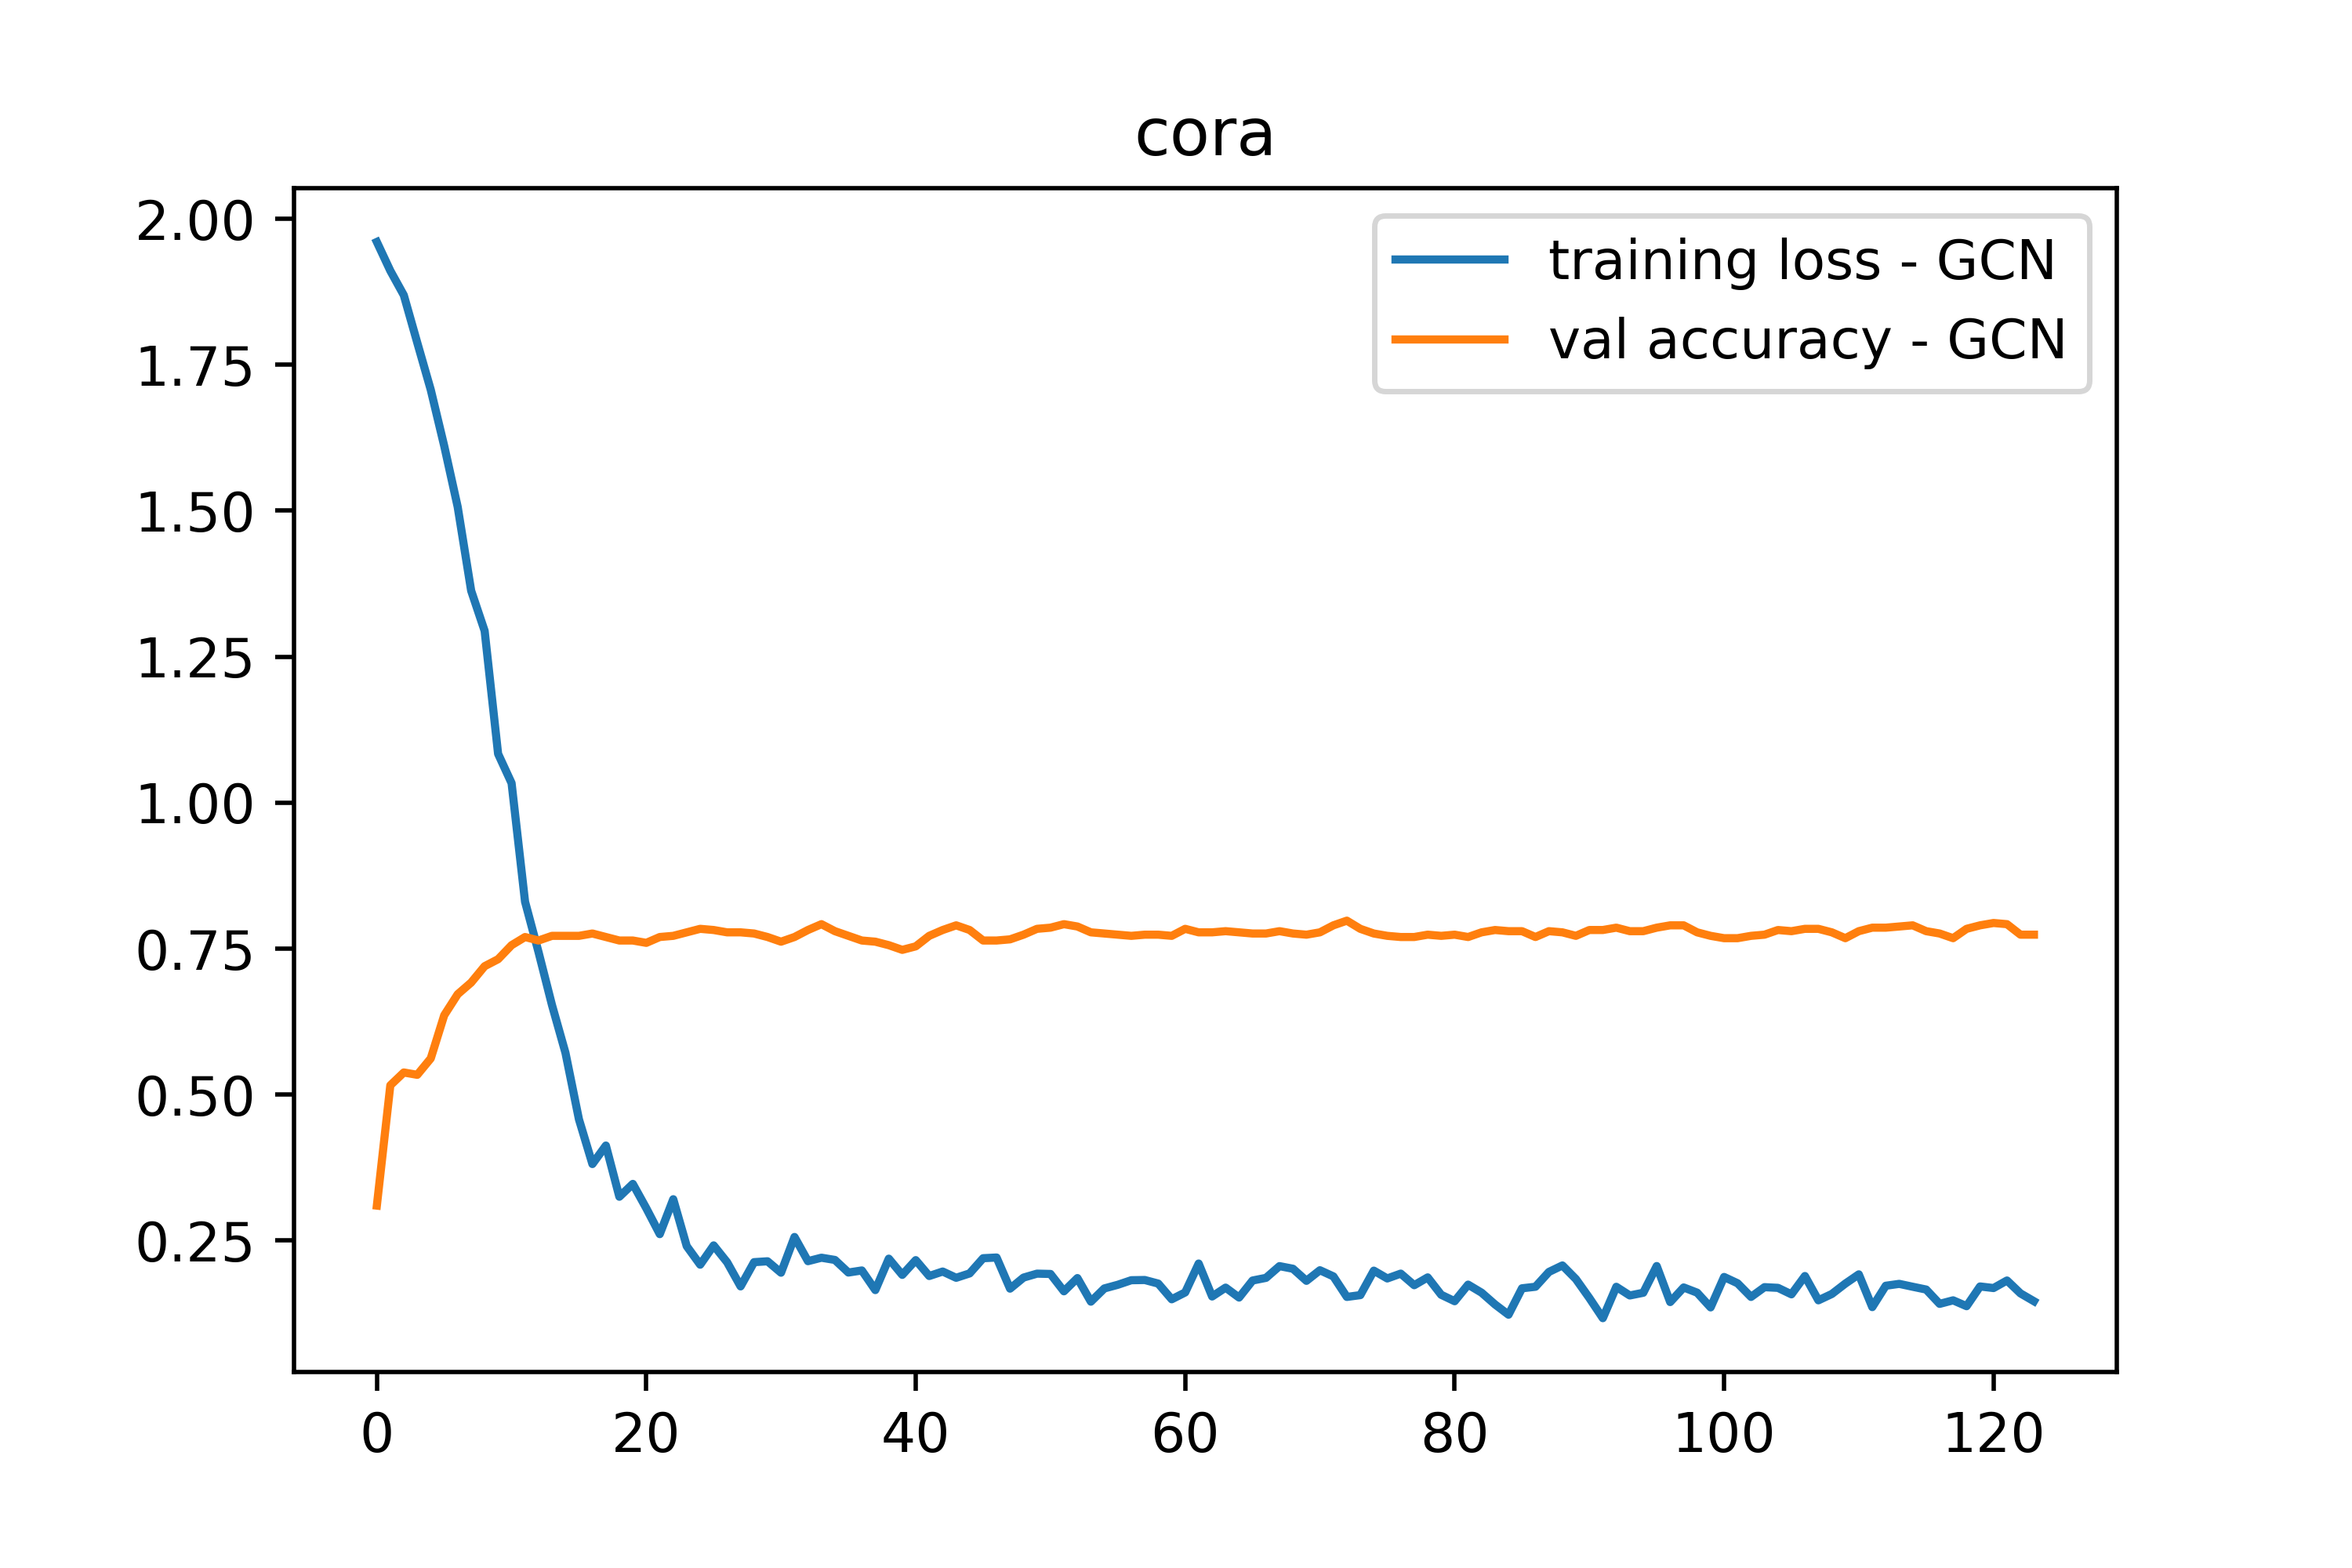
\includegraphics[width=1\linewidth]{GCN_cora_best.png}
        \end{subfigure}%
        \begin{subfigure}{0.5\linewidth}
            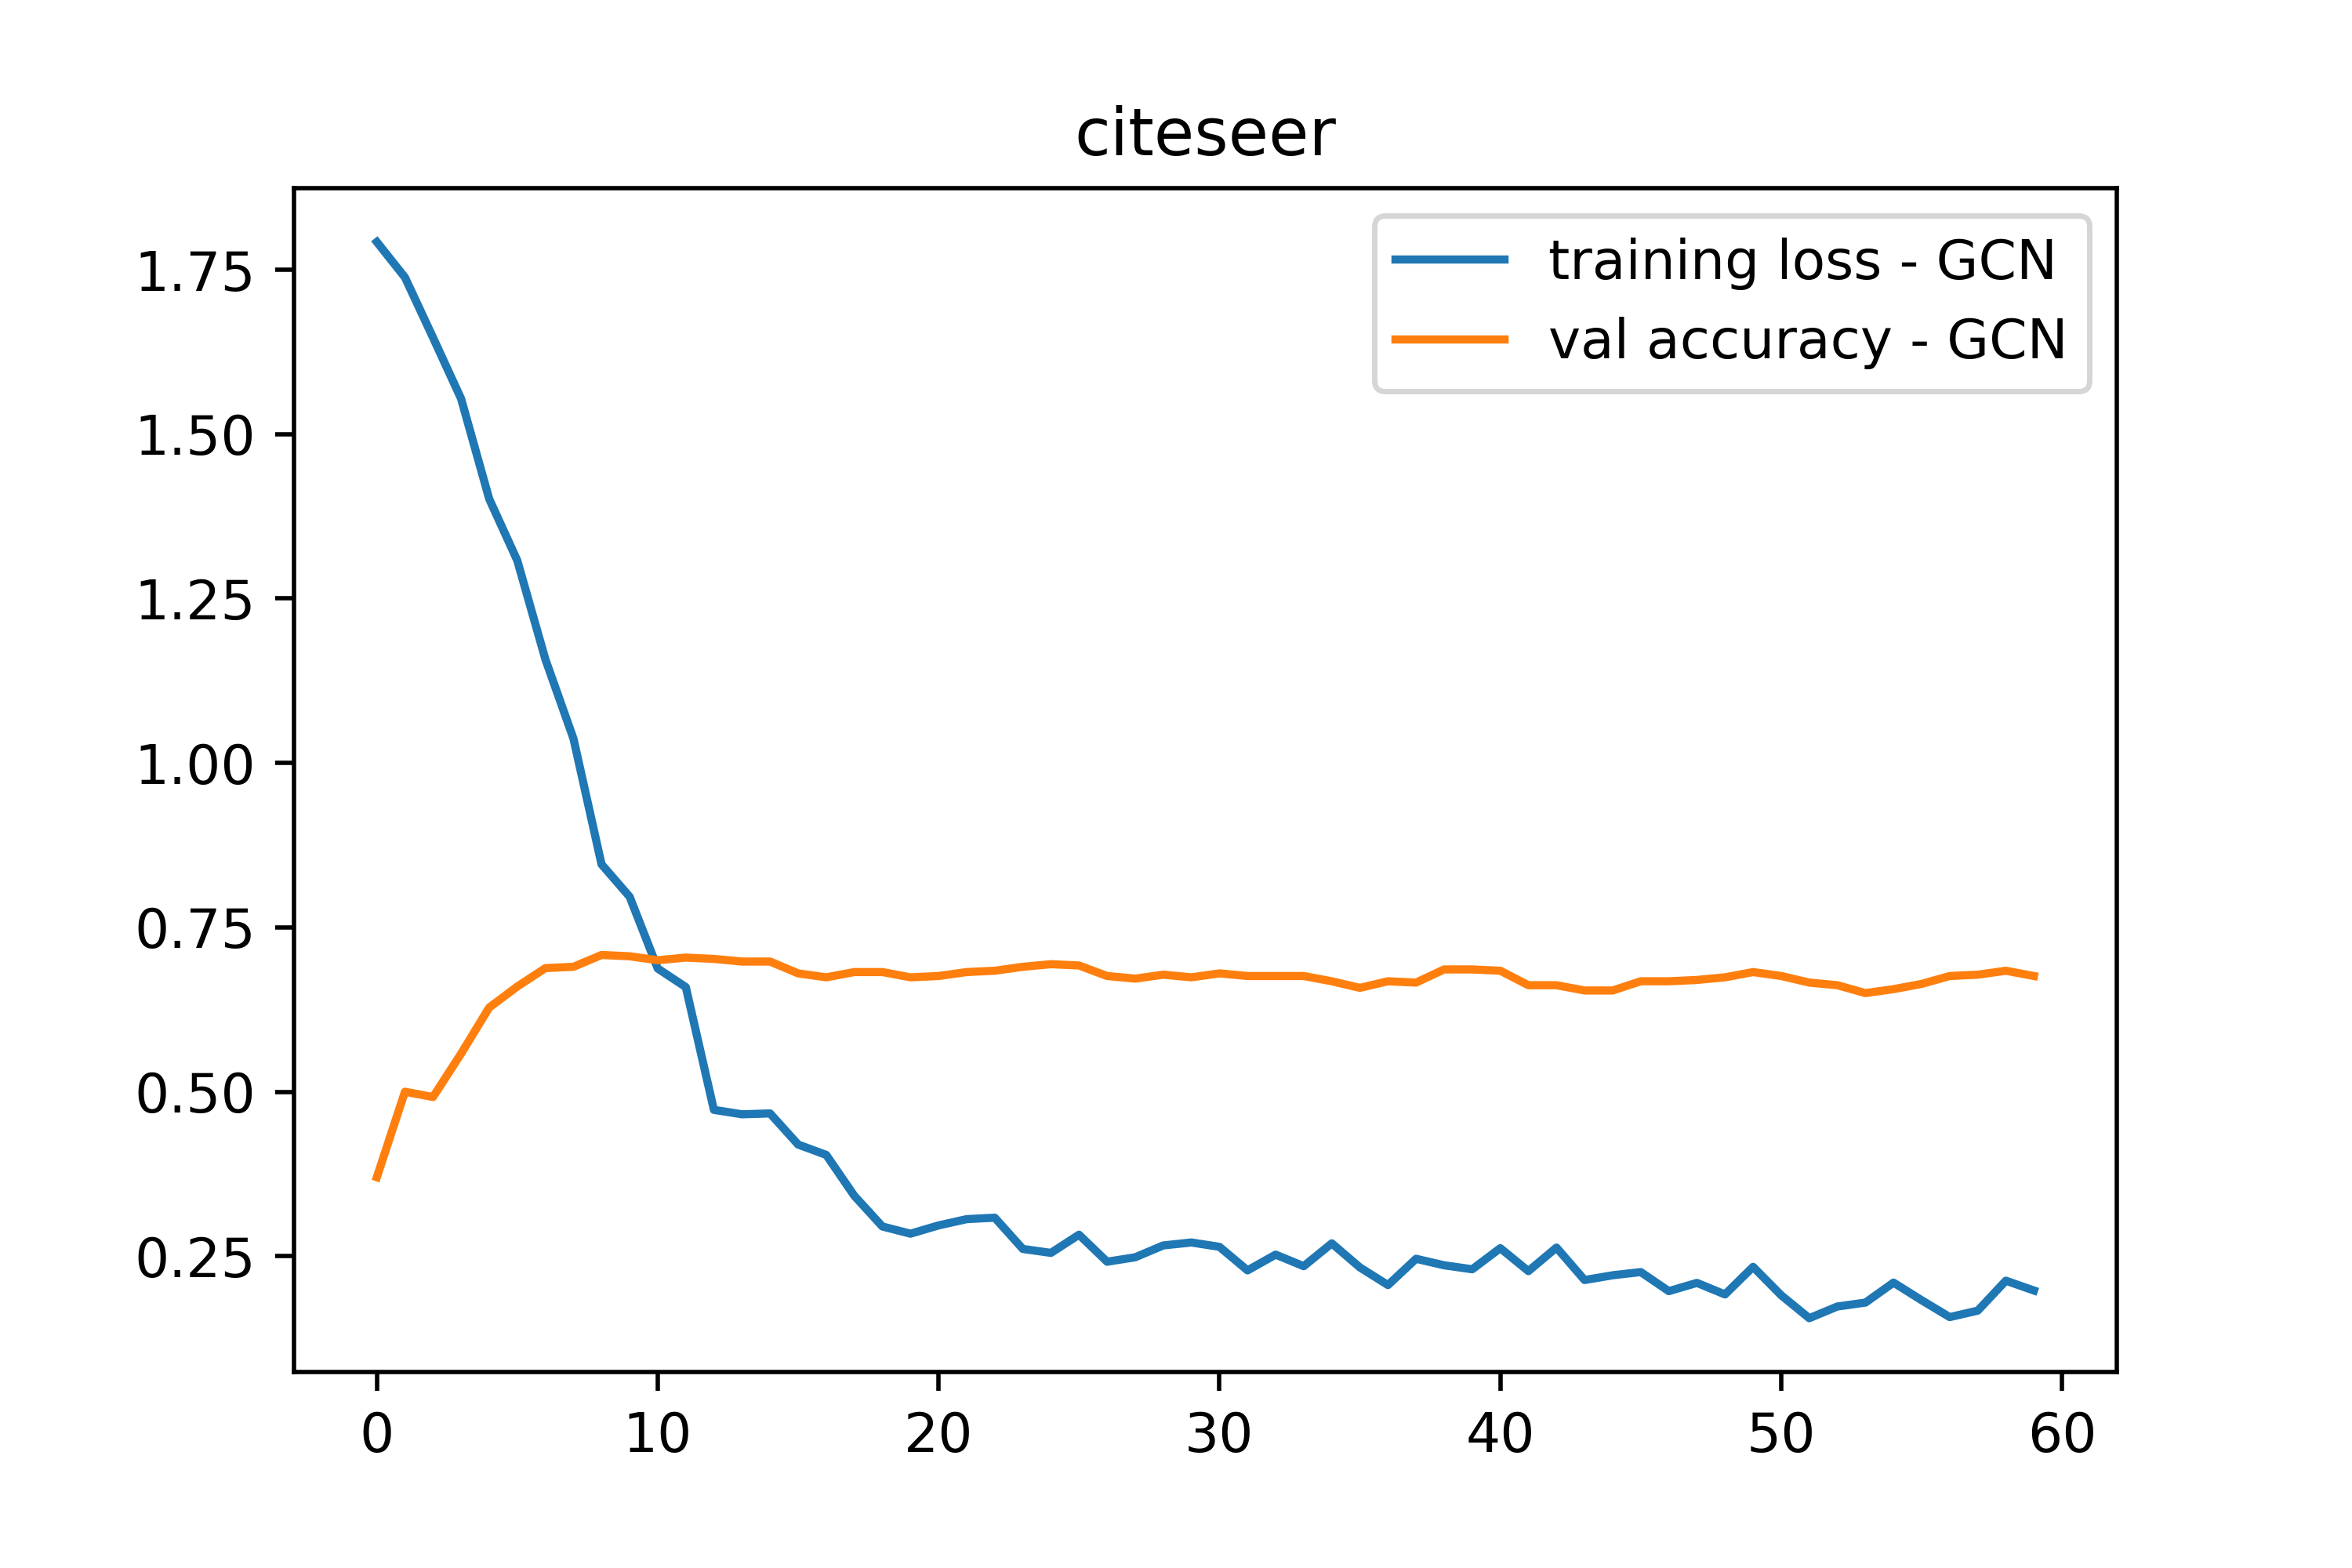
\includegraphics[width=1\linewidth]{GCN_citeseer_best.png}
        \end{subfigure}
        \caption{\textbf{GCN}. \texttt{xlabel: epochs}}
    \end{figure}%
\vspace{-0.8cm}
    \begin{figure}[H]
        \centering
        \begin{subfigure}{0.5\linewidth}
            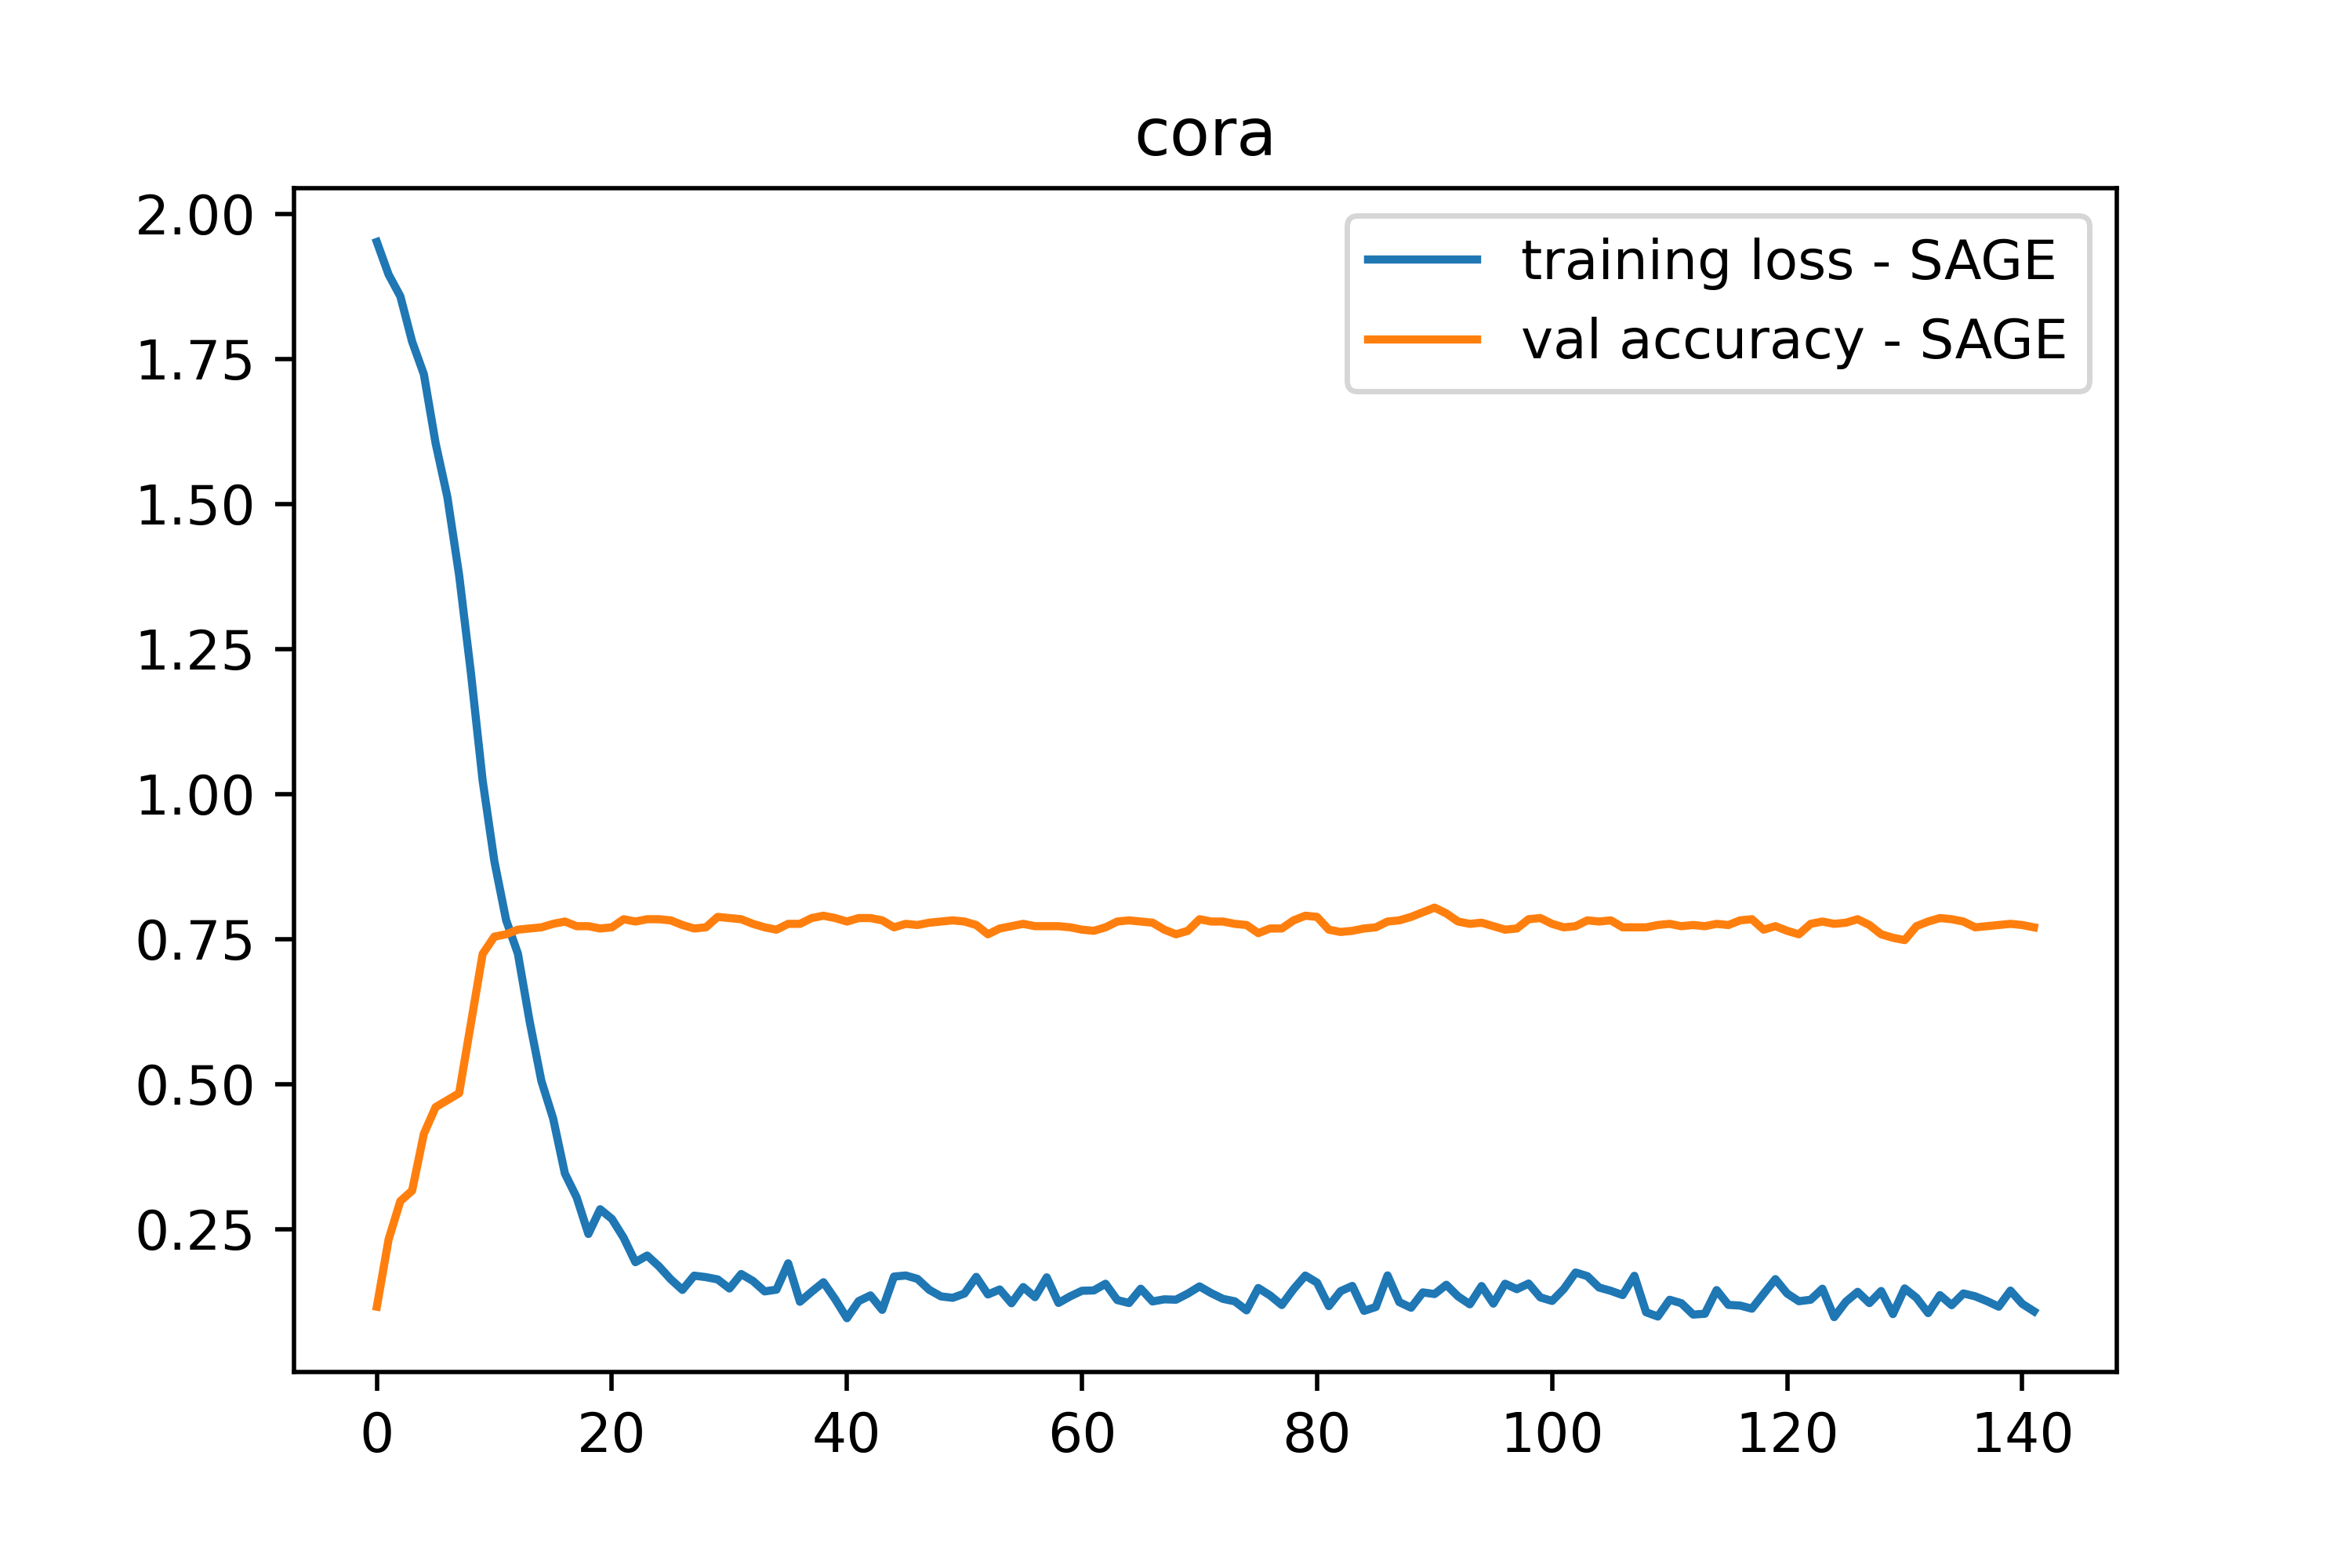
\includegraphics[width=1\linewidth]{SAGE_cora_best.png}
        \end{subfigure}%
        \begin{subfigure}{0.5\linewidth}
            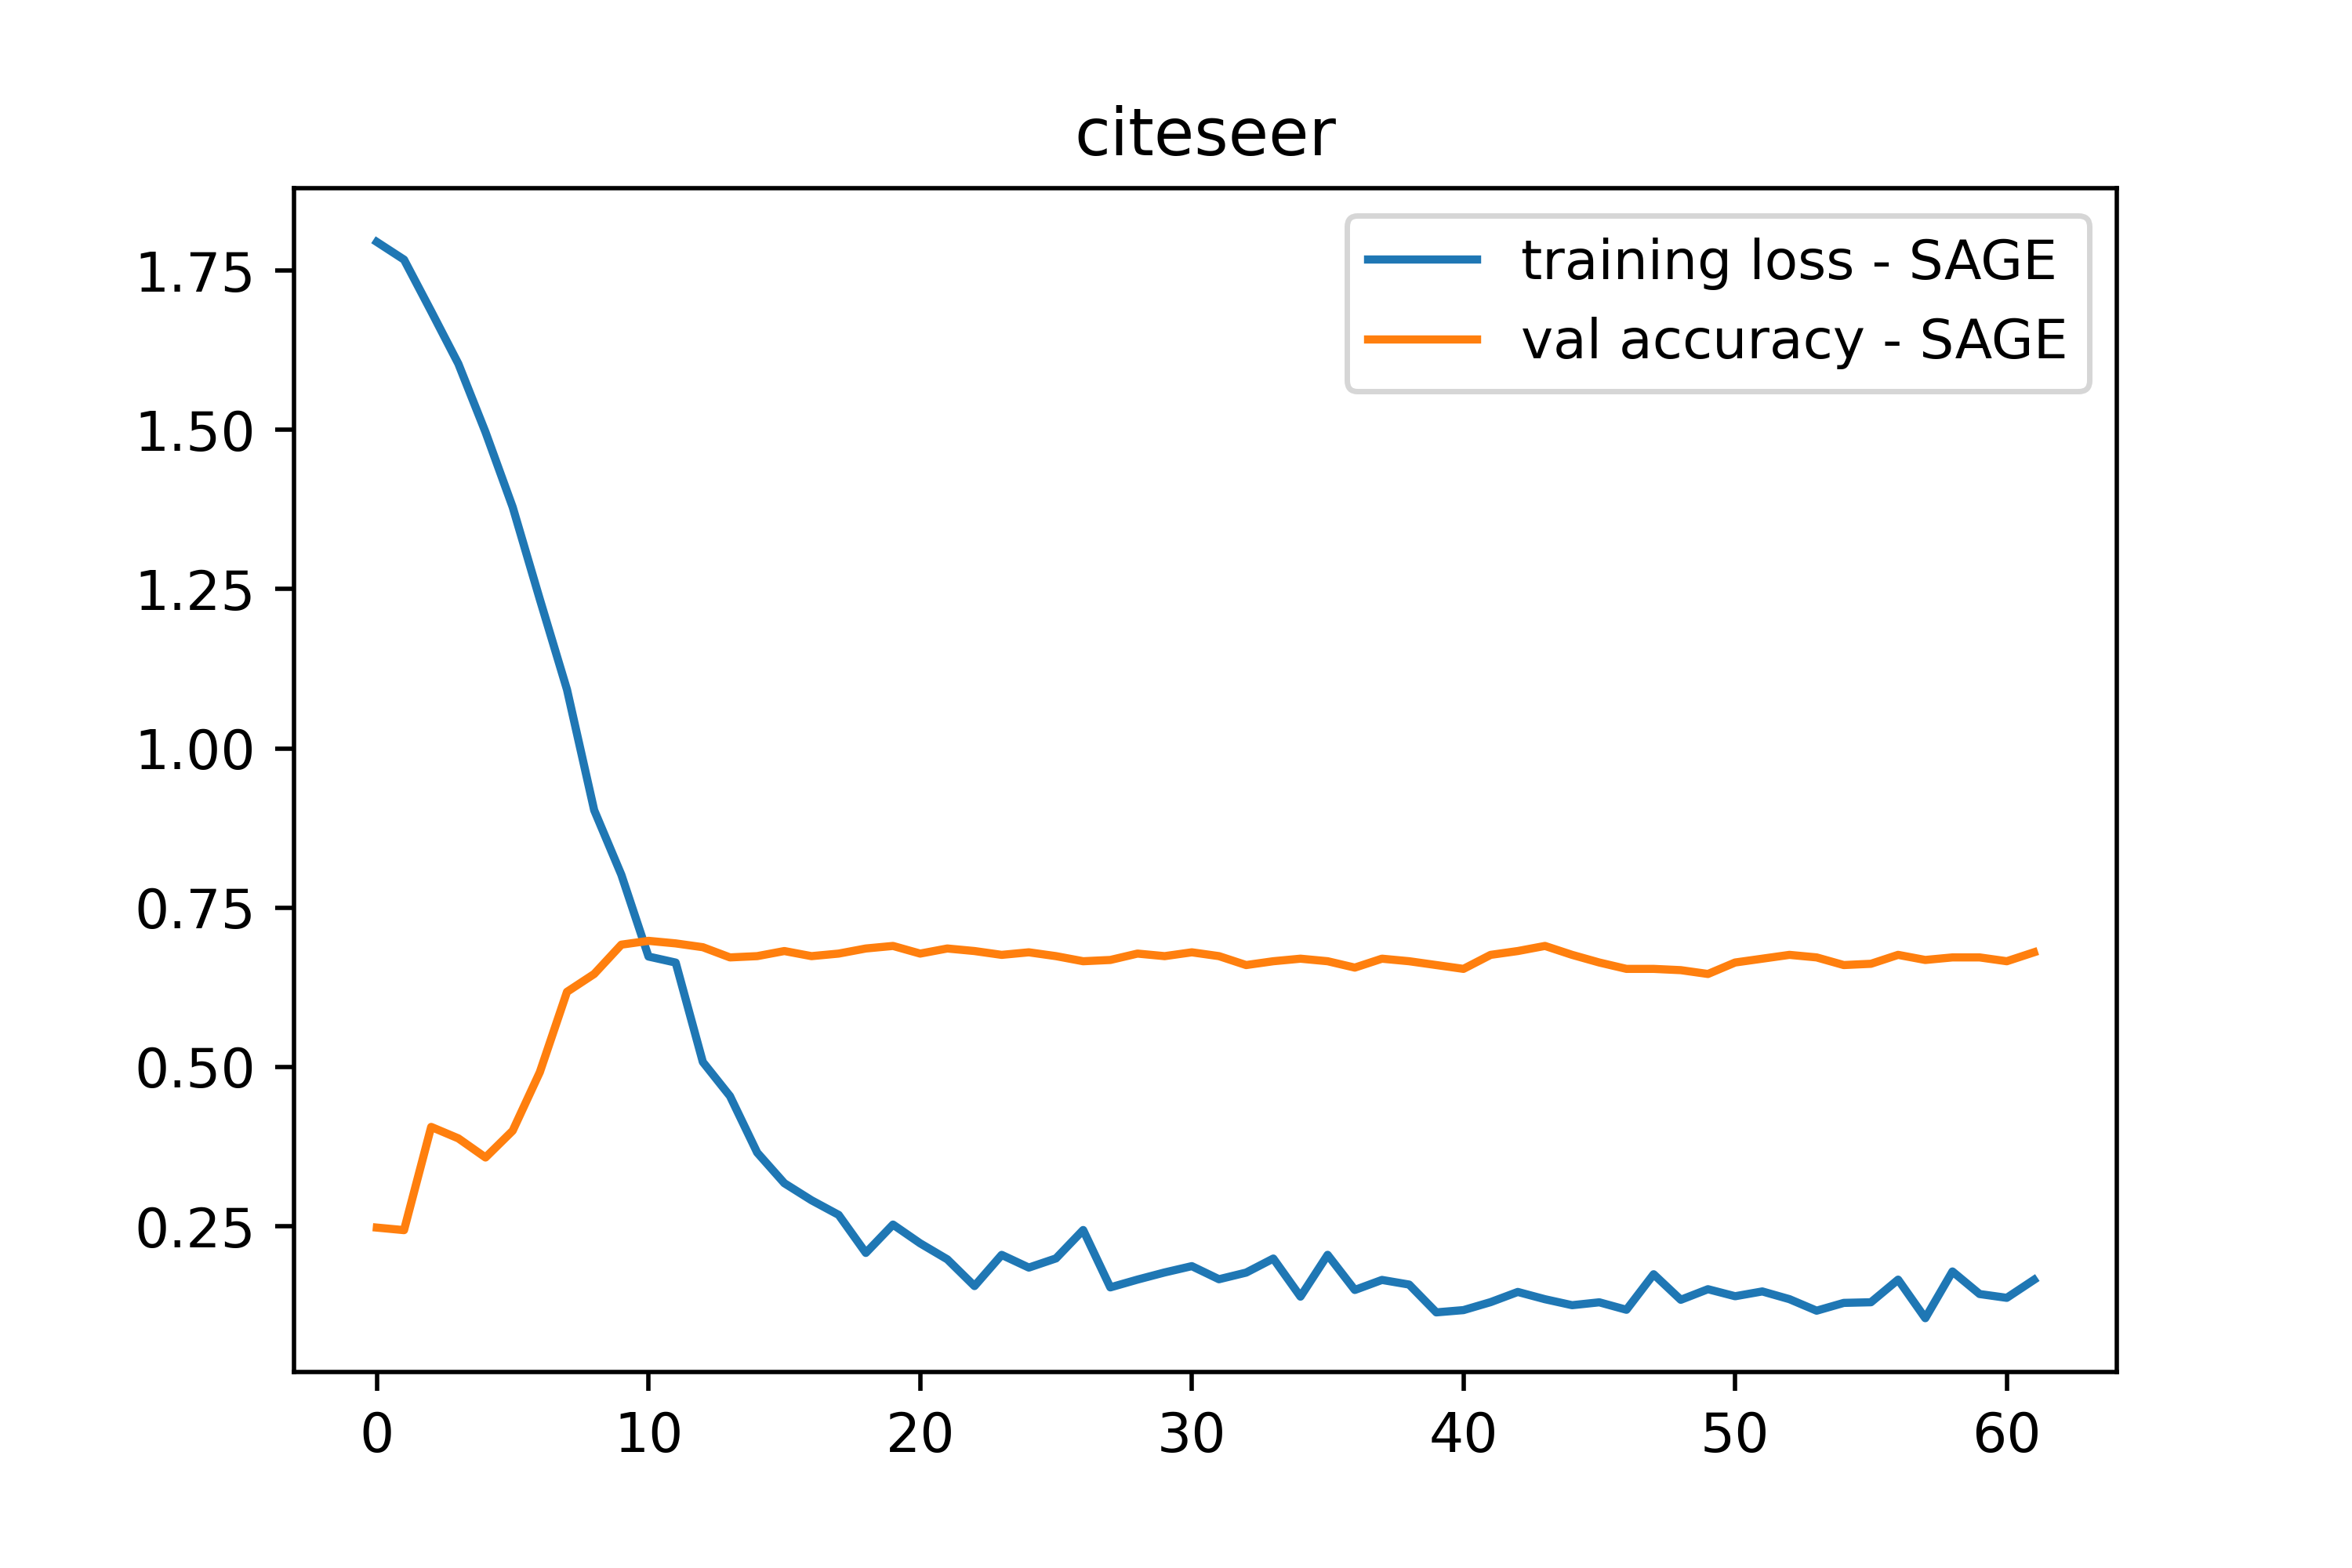
\includegraphics[width=1\linewidth]{SAGE_citeseer_best.png}
        \end{subfigure}
        \caption{\textbf{SAGE}. \texttt{xlabel: epochs}}
    \end{figure}
\vspace{-0.8cm}
    \begin{figure}[H]
        \centering
        \begin{subfigure}{0.5\linewidth}
            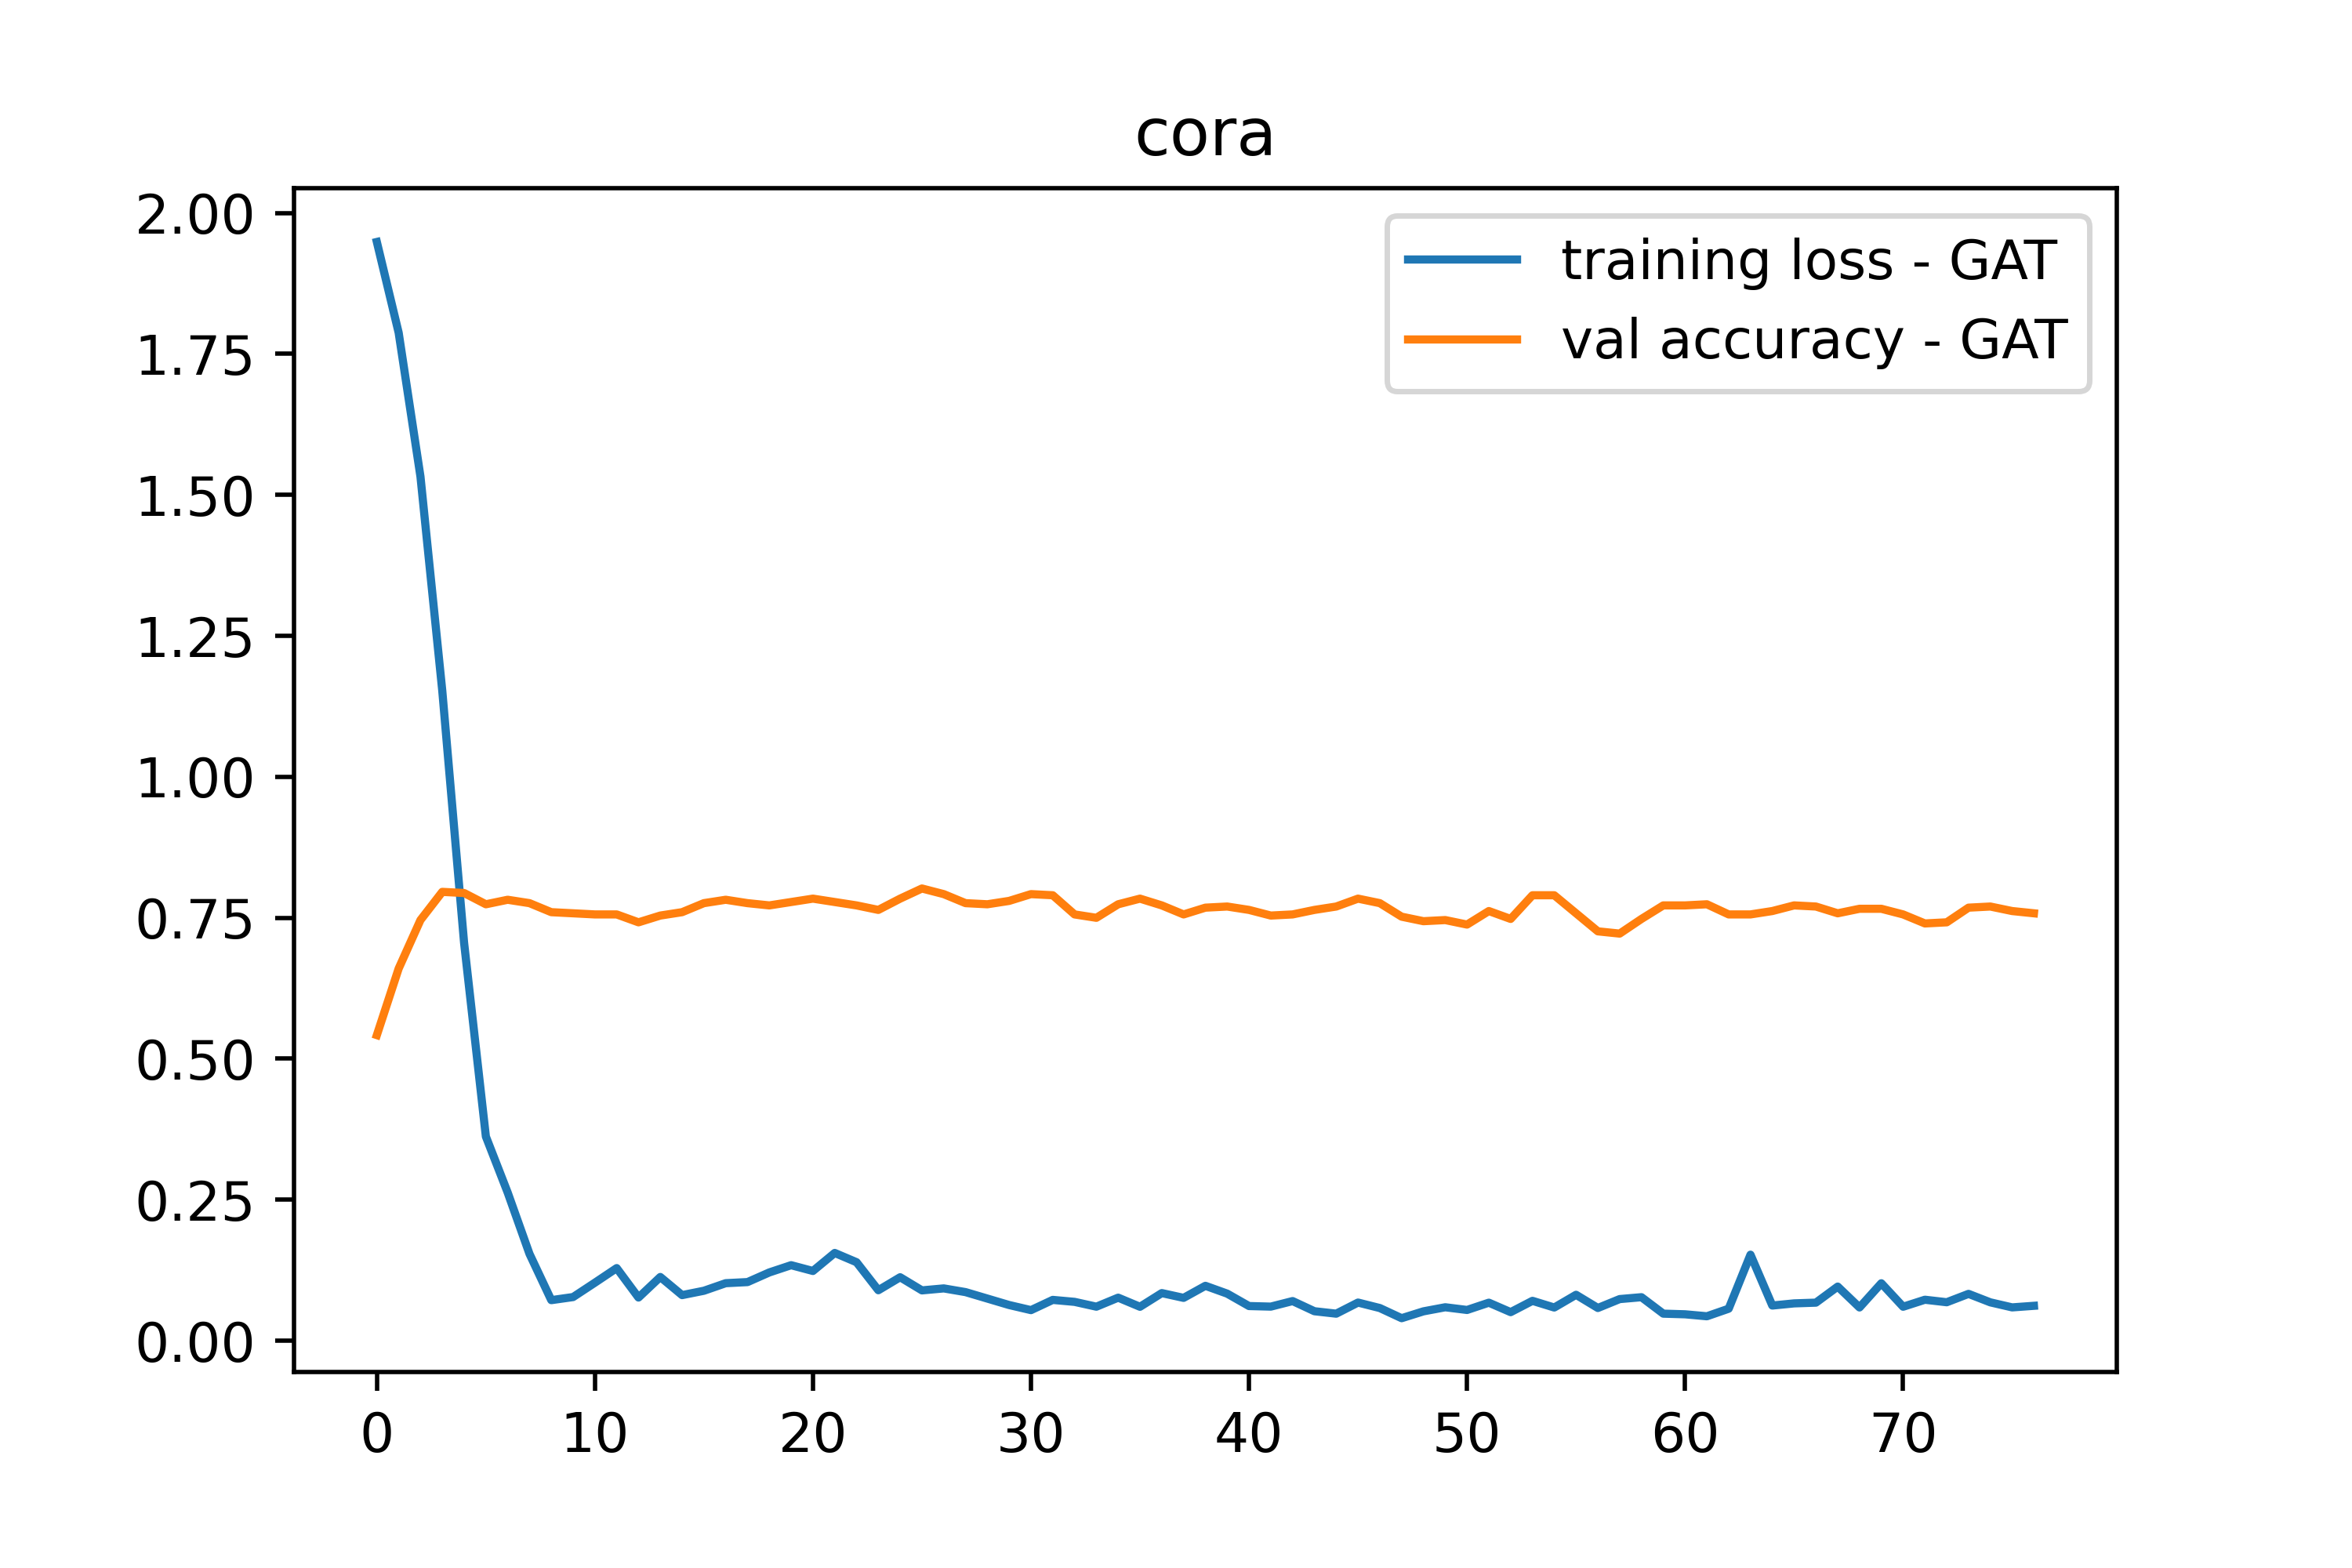
\includegraphics[width=1\linewidth]{GAT_cora_best.png}
        \end{subfigure}%
        \begin{subfigure}{0.5\linewidth}
            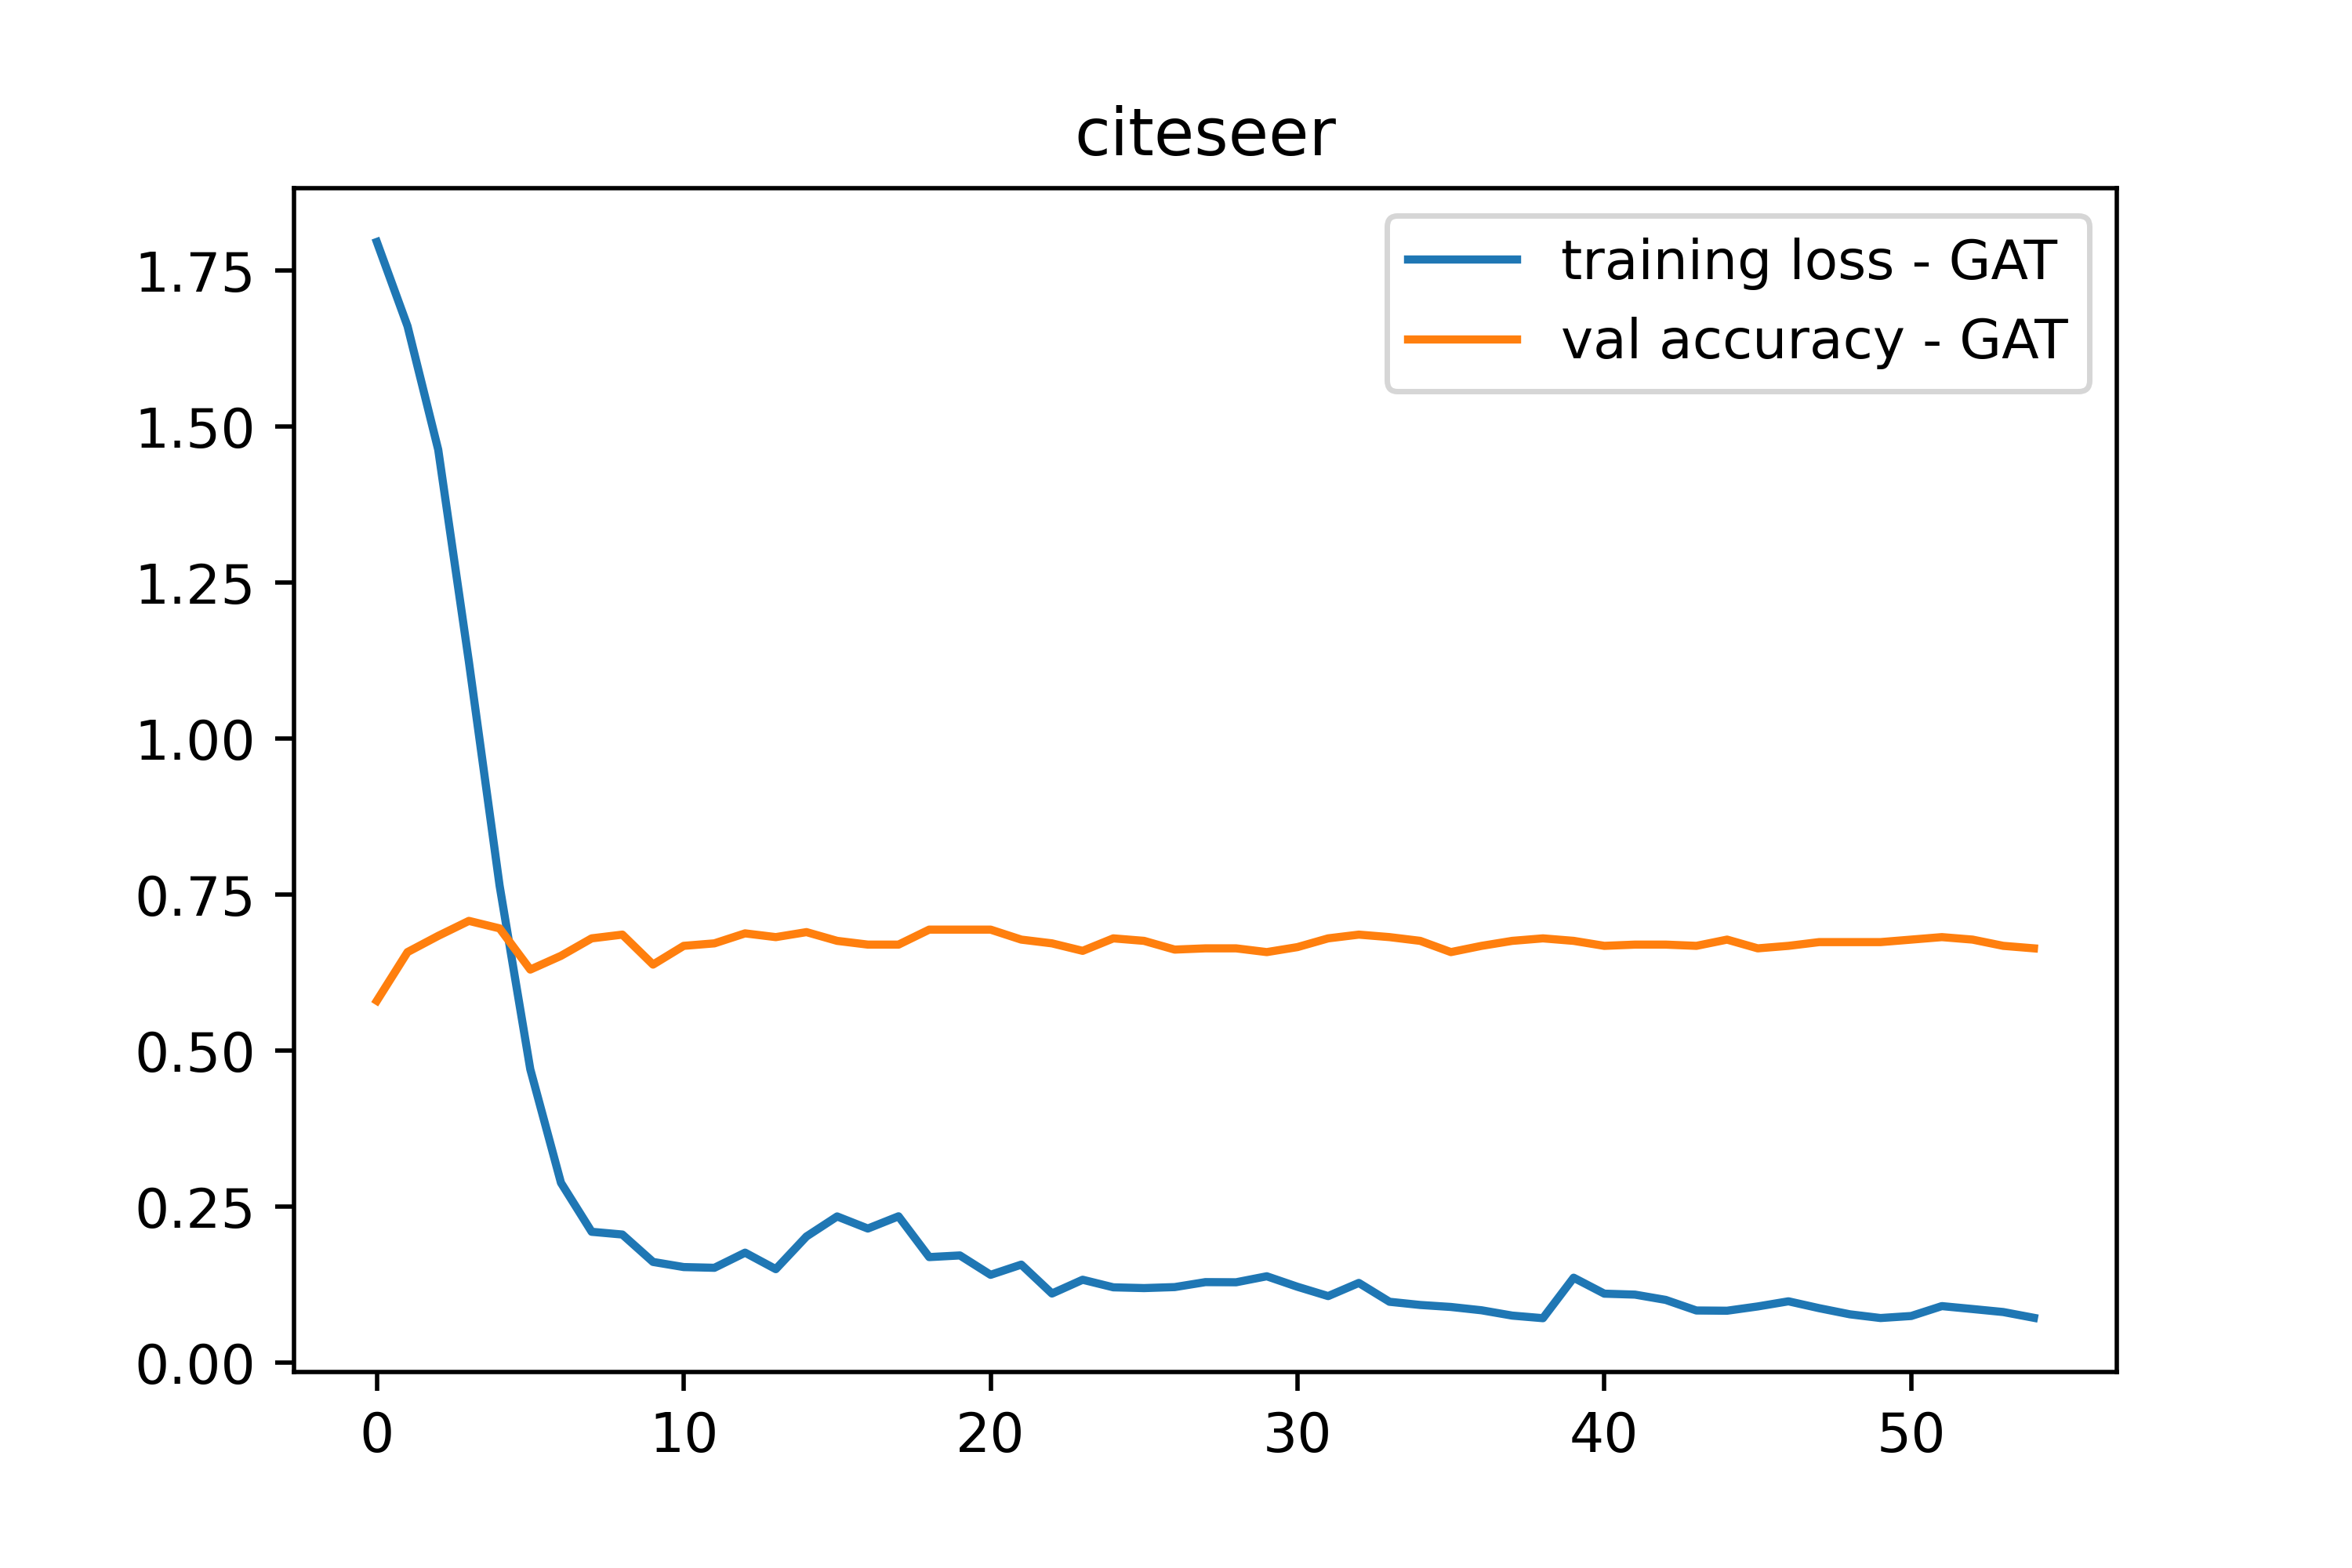
\includegraphics[width=1\linewidth]{GAT_citeseer_best.png}
        \end{subfigure}
        \caption{\textbf{GAT}. \texttt{xlabel: epochs}}
    \end{figure}
    
    \textbf{(c): } Test accuracies with the above best hyperparameters:%
\vspace{-0.4cm}
    \begin{table}[H]
        \centering
        \[\begin{array}{|c|cc|}
        \toprule
            \tikz{\node[below left, inner sep=1pt] (def) {\large \sf Model};%
                \node[above right,inner sep=1pt] (abc) {\large \sf Dataset};%
                \draw (def.north west|-abc.north west) -- (def.south east-|abc.south east);}
            & {\sf \textbf{cora}} & {\sf \textbf{citeseer}}\\
        \midrule
            {\sf GCN}  & 0.841 & 0.716 \\
            {\sf SAGE} & 0.824 & 0.684 \\
            {\sf GAT}  & 0.817 & 0.697 \\
        \bottomrule
        \end{array}\]
        \caption{Test accuracies with the above best hyperparameters}
    \end{table}
    
    
    \section{Impact on test accuracy with change in \texttt{num\_layers} and \texttt{hidden\_dim} hyperparameters}
    
    \subsection{Change in \texttt{num\_layers}}
    
    \begin{figure}[H]
        \centering
        \begin{subfigure}{0.5\linewidth}
            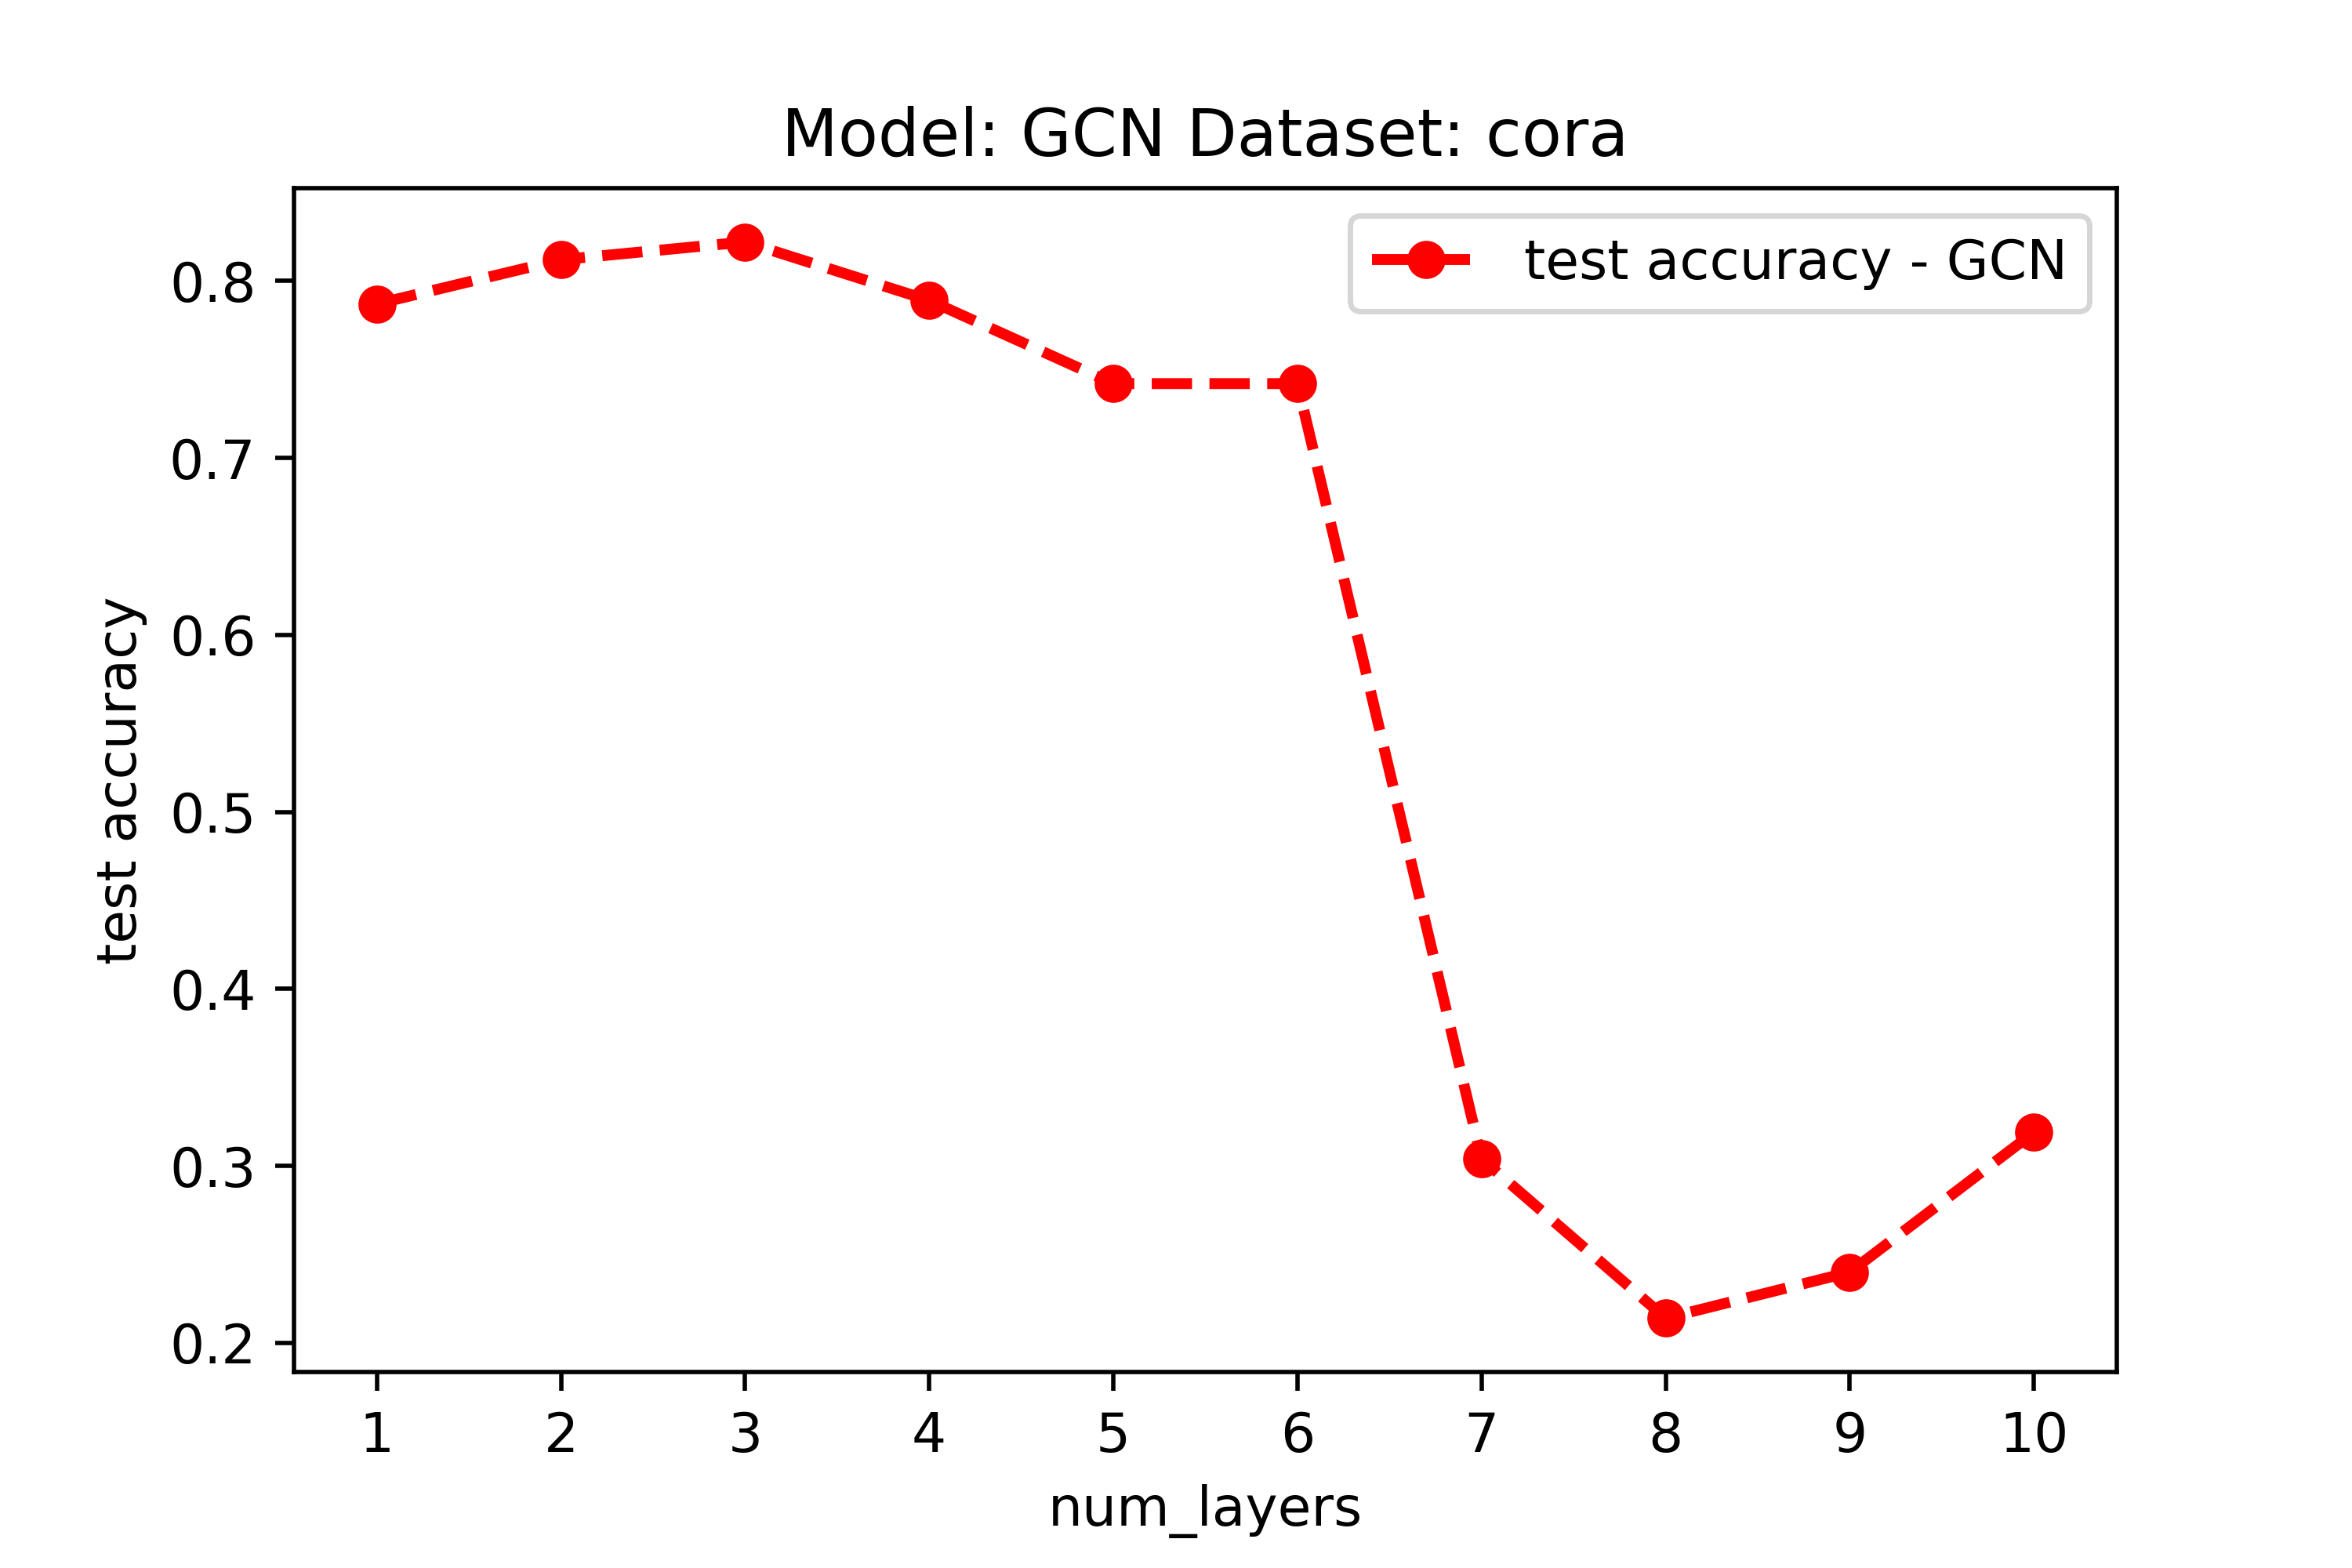
\includegraphics[width=1\linewidth]{GCN_numlayers.png}
            \caption{GCN with increase in \texttt{num\_layers}}
        \end{subfigure}%
        \begin{subfigure}{0.5\linewidth}
            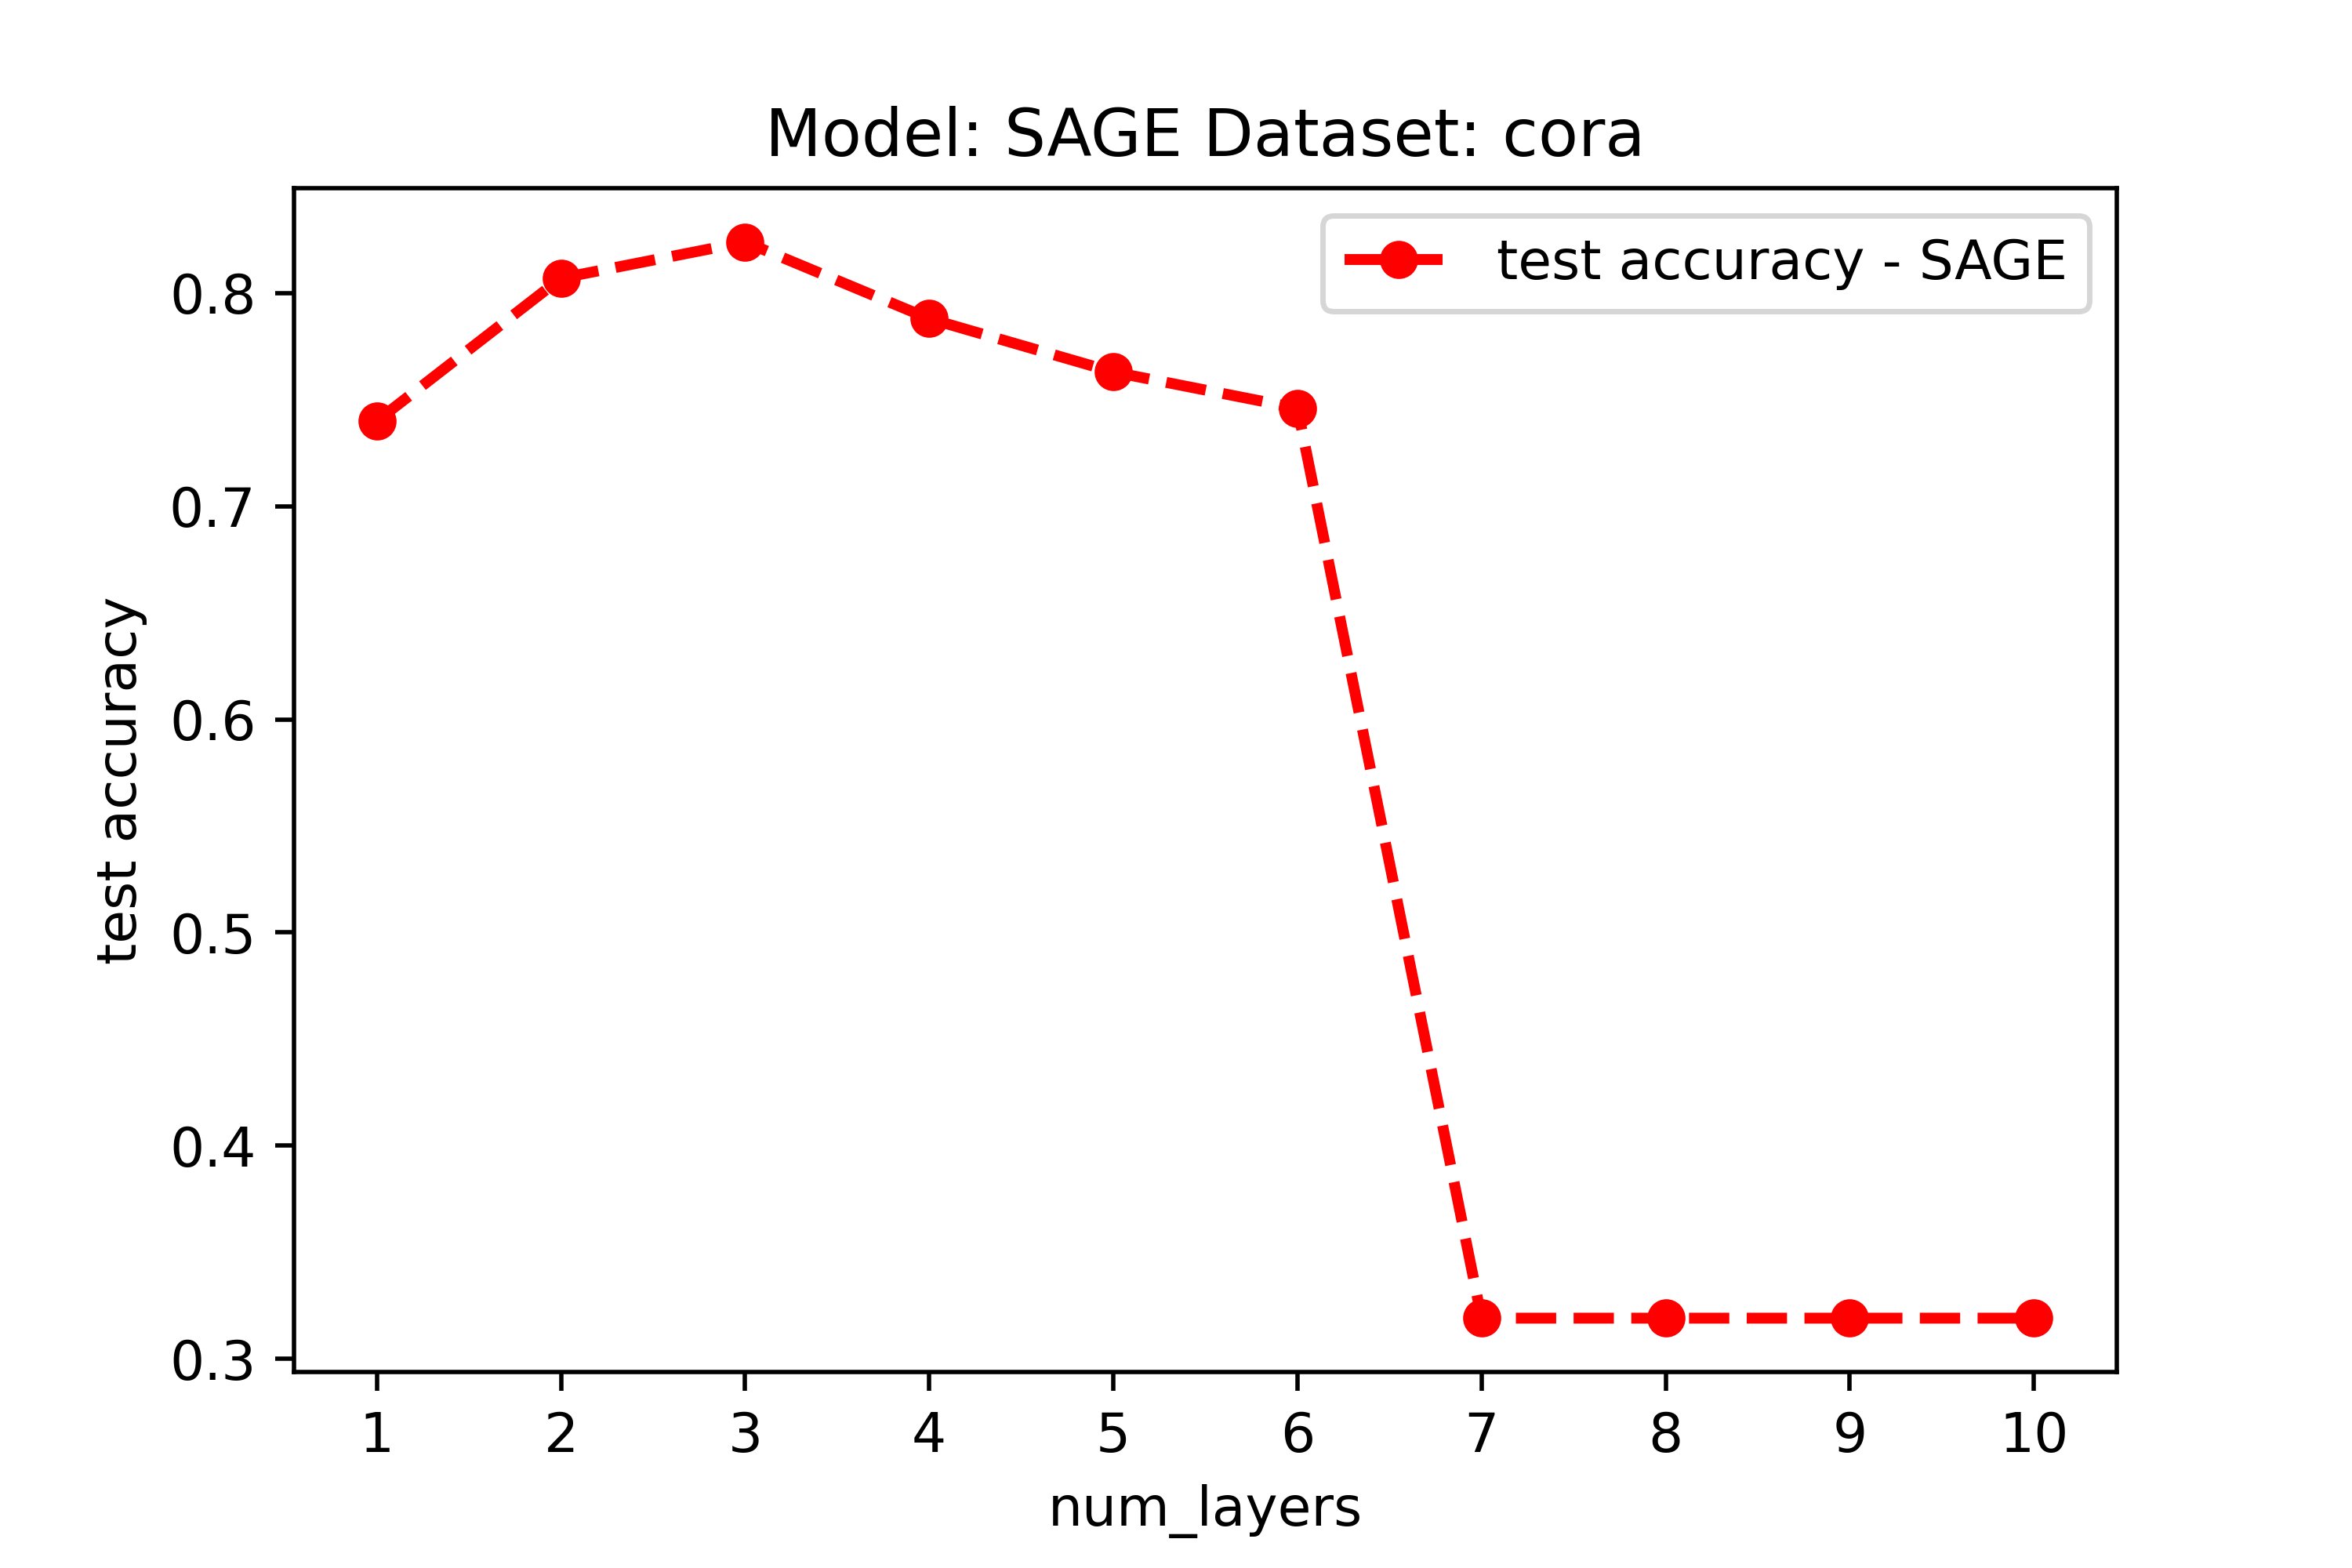
\includegraphics[width=1\linewidth]{SAGE_numlayers.png}
            \caption{SAGE with increase in \texttt{num\_layers}}
        \end{subfigure}
        \caption{Impact on test performance of models with change in the \texttt{num\_layers}.}
    \end{figure}
    
    \subsection{Change in \texttt{hidden\_dim}}
    
    \begin{figure}[H]
        \centering
        \begin{subfigure}{0.5\linewidth}
            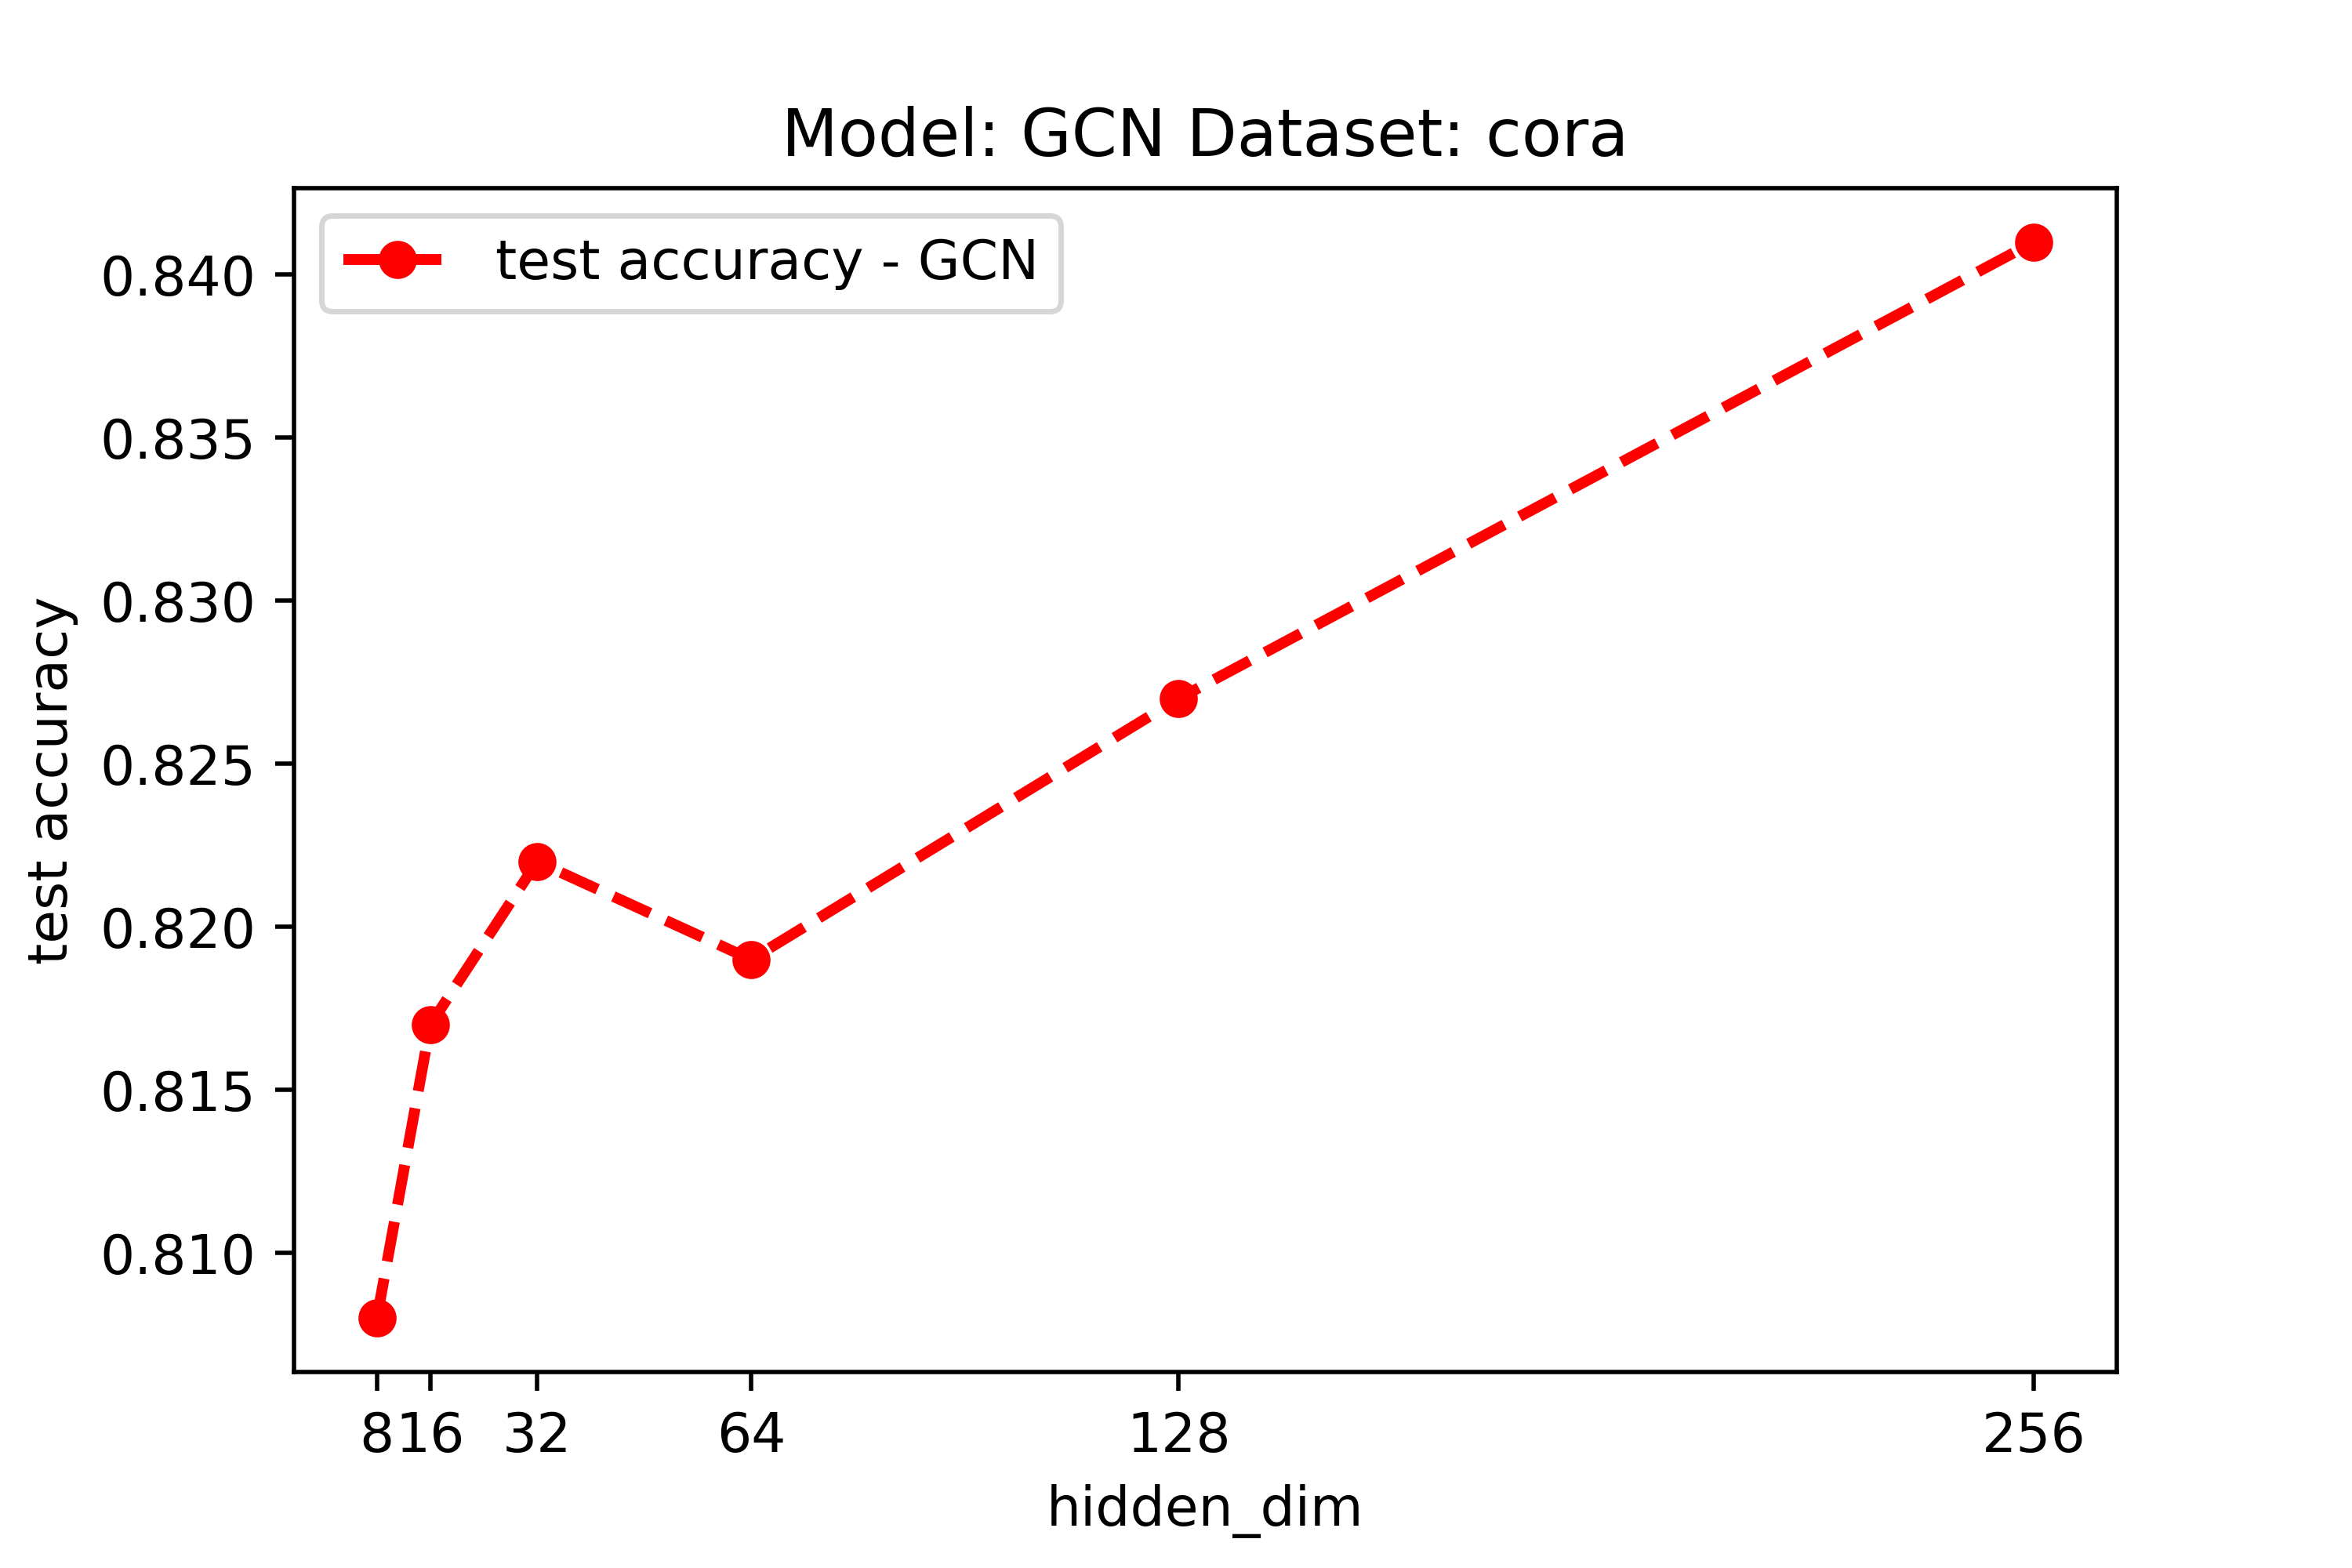
\includegraphics[width=1\linewidth]{GCN_hiddendim.png}
            \caption{GCN with increase in \texttt{hidden\_dim}}
        \end{subfigure}%
        \begin{subfigure}{0.5\linewidth}
            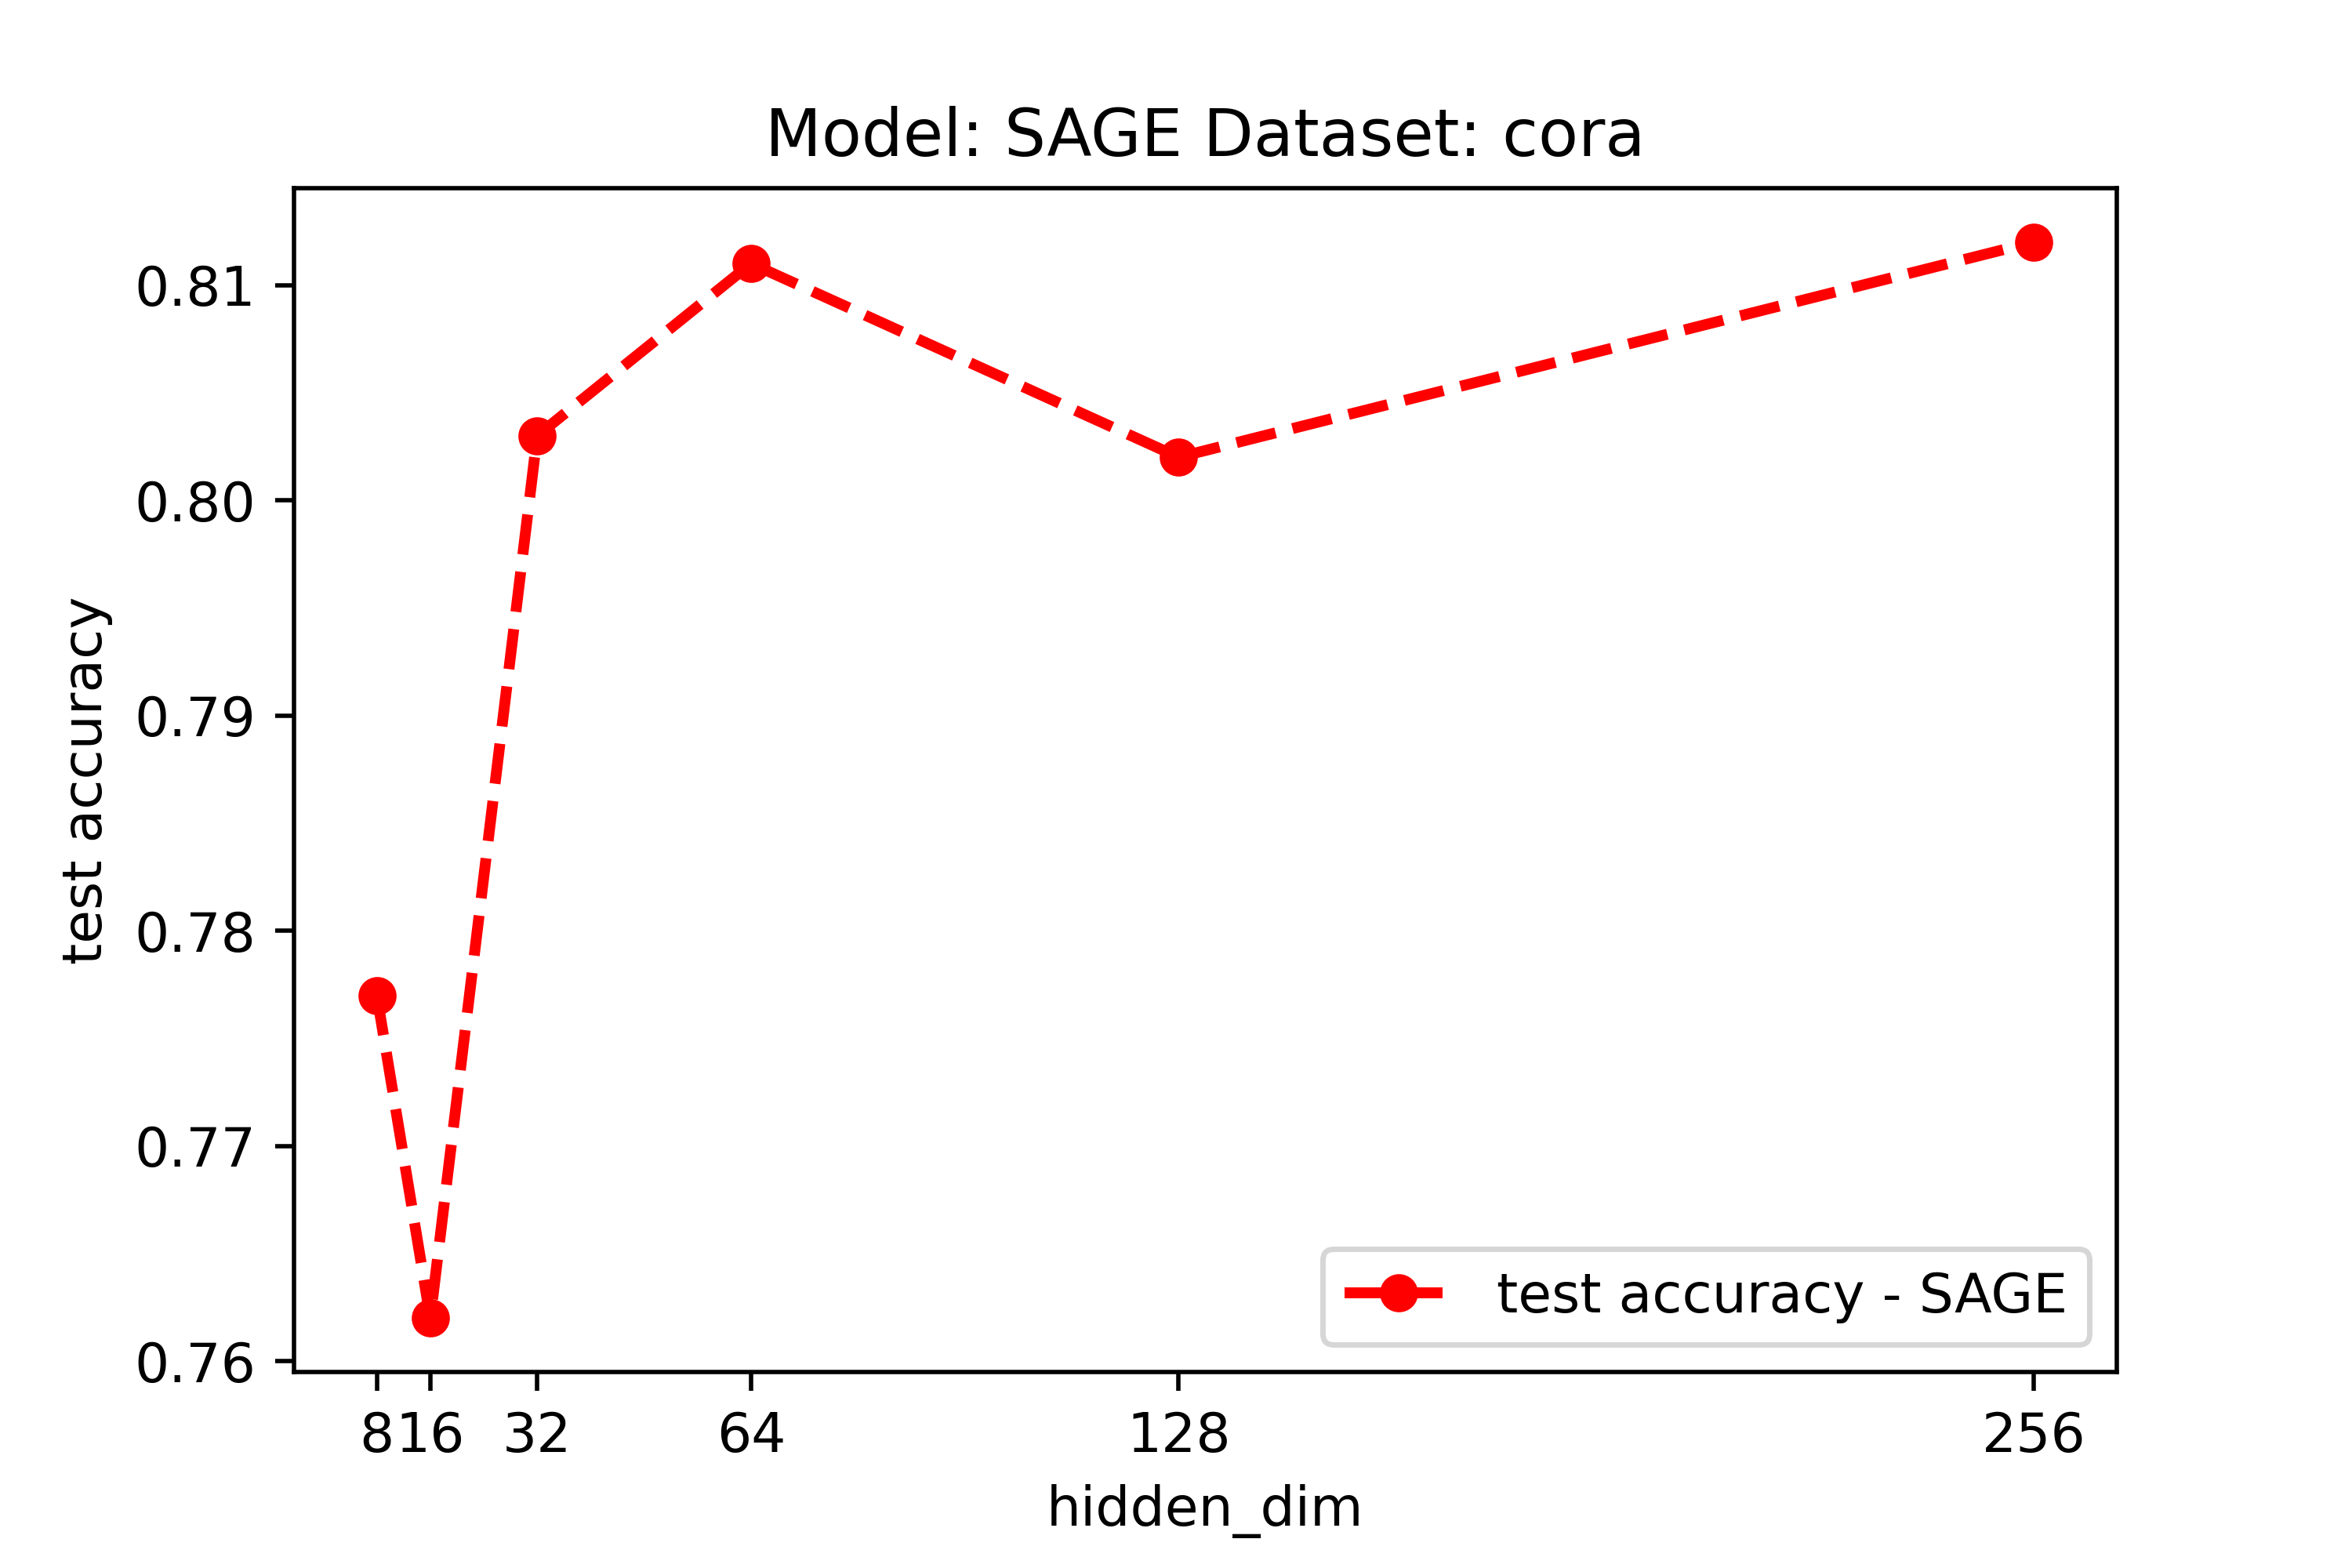
\includegraphics[width=1\linewidth]{SAGE_hiddendim.png}
            \caption{SAGE with increase in \texttt{hidden\_dim}}
        \end{subfigure}
        \caption{Impact on test performance of models with change in the \texttt{hidden\_dim}.}
    \end{figure}
    
\end{document}









